\documentclass[a4paper,german]{article}
%Mainly taken from
%https://github.com/gillescastel/university-setup/blob/master/preamble.tex
%but edited for own purposes

%%%%%OWN
%%Own basic packages
\usepackage{mkessler-math}
\usepackage{mkessler-fancythm}
\usepackage{mkessler-operators}

\usepackage{datetime}
\date{{\normalfont Mitschrift}\\{\sc Maximilian Keßler} \\ {\small Version} \\ {\small \today\; \currenttime}}

%%%%%%Preamble from Gilles Castel
% Some basic packages
\usepackage{url}
\usepackage{graphicx}
\usepackage{float}

% for wrapping text around figures
\usepackage{wrapfig}

%%This option is for now commented out, not sure what it does, but causes errors
%\pdfminorversion=7


% Don't indent paragraphs, leave some space between them
\usepackage{parskip}

% Hide page number when page is empty
\usepackage{emptypage}
% Other font I sometimes use.
\usepackage{xcolor}
% \usepackage{cmbright}

% Math stuff
\usepackage{amsfonts}

% Put x \to \infty below \lim
\let\svlim\lim\def\lim{\svlim\limits}

%Make implies and impliedby shorter
\let\implies\Rightarrow
\let\impliedby\Leftarrow
\let\iff\Leftrightarrow
\let\epsilon\varepsilon

% Command for short corrections
% Usage: 1+1=\correct{3}{2}

% Environments
\makeatother

% Fix some spacing
% http://tex.stackexchange.com/questions/22119/how-can-i-change-the-spacing-before-theorems-with-amsthm
\makeatletter
\def\thm@space@setup{%
  \thm@preskip=\parskip \thm@postskip=0pt
}


% \lecture starts a new lecture (les in dutch)
%
% Usage:
% \lecture{1}{di 12 feb 2019 16:00}{Inleiding}
%
% This adds a section heading with the number / title of the lecture and a
% margin paragraph with the date.

% I use \dateparts here to hide the year (2019). This way, I can easily parse
% the date of each lecture unambiguously while still having a human-friendly
% short format printed to the pdf.

\usepackage{xifthen}
\def\testdateparts#1{\dateparts#1\relax}
\def\dateparts#1 #2 #3 #4 #5\relax{
    \marginpar{\small\textsf{\mbox{#1 #2 #3 #5}}}
}

\def\@lecture{}%
\newcommand{\lecture}[3]{
    \ifthenelse{\isempty{#3}}{%
    \def\@lecture{\ifenglish Lecture\else Vorlesung\fi\, #1}%
    }{%
\def\@lecture{\ifenglish Lecture\else Vorlesung\fi\, #1: #3}%
    }%
    \subsection*{\@lecture}
    \marginpar{\small\textsf{\mbox{#2}}}
}

% These are the fancy headers
\usepackage{fancyhdr}
\pagestyle{fancy}

% LE: left even
% RO: right odd
% CE, CO: center even, center odd
% My name for when I print my lecture notes to use for an open book exam.
% \fancyhead[LE,RO]{Gilles Castel}

\fancyhead[RO,LE]{\@lecture} % Right odd,  Left even
\fancyhead[RE,LO]{}          % Right even, Left odd

\fancyfoot[RO,LE]{\thepage}  % Right odd,  Left even
\fancyfoot[RE,LO]{}          % Right even, Left odd
\fancyfoot[C]{\leftmark}     % Center

\makeatother

% Todonotes and inline notes in fancy boxes
\usepackage{todonotes}

% Make boxes breakable
\tcbuselibrary{breakable}

% Figure support as explained in my blog post.
\usepackage{import}
\usepackage{xifthen}
\usepackage{pdfpages}
\usepackage{transparent}
\newcommand{\incfig}[1]{%
    \def\svgwidth{\columnwidth}
    \import{./figures/}{#1.pdf_tex}
}

% Fix some stuff
% %http://tex.stackexchange.com/questions/76273/multiple-pdfs-with-page-group-included-in-a-single-page-warning
\pdfsuppresswarningpagegroup=1






\title{{Einführung in die} \\ Geometrie und Topologie}
\author{{\normalfont Dozent}\\{\sc Dr. Daniel Kasprowski}}

\renewcommand\subset\subseteq
%\DeclareMathOperator{\Topo}{O}
\def\Topo{\mathcal{O}}

\begin{document}
    \maketitle
    \section{testing}
    ref : \ref{thm:heine-borel}, \\
nameref:    \nameref{thm:heine-borel}\\
autoref: \autoref{thm:heine-borel} \\
cref: \cref{thm:heine-borel} \\
ref: \ref{thm:point-in-hausdorff-space-is-closed} \\
autoref:    \autoref{thm:point-in-hausdorff-space-is-closed} \\
cref:    \cref{thm:point-in-hausdorff-space-is-closed} \\
nameref:    \nameref{thm:point-in-hausdorff-space-is-closed} \\
\listoftheorems
    \tableofcontents
    % start lectures
    %! TEX root = ./master.tex
\lecture[Metrische Räume. Umgebungen, offene Mengen, Stetigkeit. Topologische Räume. Metrisierbarkeit.]{Di 13 Apr 2021 12:16}{Einführung}
\begin{orga}
\begin{itemize}
\item    Die Vorlesung wird aufgezeichnet.
\item Wir duzen uns.
\item Für die Übungen muss man sich auf eCampus anmelden, ob Do, 20:00 Uhr (Do 15 Apr 2021 20:00 Uhr)
\item Die Übungsblätter werden Donnerstag zur Verfügung gestellt und werden nach 10 Tagen am Montag, 10 Uhr abgegeben.
\item Es wird eine Fragestunde um Donnerstag, 16 Uhr geben.
\item Es wird kein Skript geben, allerdings werden die geschriebenen Notizen auf eCampus zur Verfügung gestellt.
\item Die Vorlesung orientiert sich an der vom letzten Jahr.
\item Für Literatur sind empfohlen: \cite{topology-waldhausen}, \cite{algebraic-topology-hatcher} sowie \cite{topology-and-geometry} (auch auf der Vorlesungshomepage zu finden).
\end{itemize}
\end{orga}

\setcounter{section}{-1}

\section{Motivation und Überblick}
In der Topologie studieren wir topologische Räume. Diese verallgemeinern metrische Räume. Wir wollen zwei metrische Räume $X,Y$ als 'gleich' ansehen, wenn es stetige, zueinander inverse Abbildungen  $X \to  Y, Y\to X$ gibt.
\begin{example}
    Betrachte ein Quadrat und einen Kreis, wir können sie durch Streckung aufeinander abbilden. Gleiches gilt für eine Tasse und einen Donut. \\
    \begin{minipage}{\textwidth}
    \centering
    \begin{minipage}{0.45\textwidth}
     \incfig{quadrat-und-kreis-sind-gleich}
    \end{minipage}
    \begin{minipage}{0.45\textwidth}
    \incfig{tasse-und-donut-sind-gleich}
    \end{minipage}
    \captionof{figure}{Beispiele 'gleicher' metrischer Räume (homöomorph)}
\end{minipage}
\end{example}




\begin{idea}
    Räume sind gewissermaßen aus 'Knete'.
\end{idea}
\begin{goal}
    Wann sind zwei Räume gleich?
\end{goal}
Dazu werden wir algebraische Invarianten verwenden.
\begin{example}
    $\R^n$ und $\R^m$ sind nicht 'gleich' für $n\neq m$.
\end{example}
Der Aufbau ist wie folgt:
\begin{description}
    \item[1. Teil] Grundlagen
    \item[2. Teil] erste Invarianten: Fundamentalgruppe (dazu Überlagerungen)
\end{description}


\newpage
\part{Mengentheoretische Topologie}

\section{Metrische Räume}
\begin{definition}[Metrik]\label{def:metrik}
    Eine \vocab[Metrik]{Metrik} auf einer Menge $X$ ist eine Funktion  $d: X\times X \to  \R_{\geq 0}$ mit folgenden Eigenschaften:
    \begin{enumerate}[(i)]
        \item $d(x,y) = 0 \iff  x = y$
        \item $d(x,y) = d(y,x) \quad \forall x,y\in X$
        \item (Dreiecksungleichung) $d(x,z) \leq  d(x,y) + d(y,z)$.
    \end{enumerate}
    Ein \vocab{Metrischer Raum} ist ein Paar $(X,d)$ aus einer Menge $X$ und einer Metrik $d$ auf $X$.
\end{definition}

\begin{definition}[Stetigkeit]\label{def:stetig-metrischer-raum}
    Seien $(X,d)$ und  $(X',d')$ zwei metrische Räume. Dann ist eine Funktion $f:X \to  Y$ \vocab[Stetig!in $x\in X$]{stetig in $x\in X$}, falls
    \[
        \forall ε > 0 \; \exists \delta > 0 \; \forall x' \colon d(x,x') < \delta \implies d'(f(x), f(x')) < ε
    .\] 
    Eine Funktion $f$ heißt \vocab[Stetig]{stetig}, wenn sie in jedem Punkt  $x\in X$ stetig ist.
    \begin{minipage}{\textwidth}
        \centering
    \incfig{definition-von-stetigkeit-in-metrischen-raeumen}
    \captionof{figure}{Definition von Stetigkeit in metrischen Räumen}
    \end{minipage}
\end{definition}


\begin{example}
    \begin{itemize}
        \item 
    Sei $V$ ein reeller Vektorraum mit Norm  $\lVert \cdot  \rVert$. Dann definiert
    \[
        d(v,w) := \lVert v-w \rVert 
    .\] 
    eine Metrik auf $V$. Insbesondere ist $\R^n$ mit euklidischer Norm
    \[
        \lVert (x_1,\ldots,x_n) \rVert _2 = \sqrt{x_1^2 + \ldots + x_{n}^2} 
    .\] 
    dadurch ein metrischer Raum.
\item Ist $(X,d)$ ein metrischer Raum und  $Y\subset X$ eine Teilmenge, dann ist $(Y, d| _{Y\times Y})$ ein metrischer Raum.
\item Sei $X$ eine Menge. Dann ist
    \[
        d(x,y) = \begin{cases}
            0 & \text{falls } x=y \\
            1 & \text{sonst}
        \end{cases}
    .\] 
    eine Metrik auf $X$, genannt die \vocab[Metrik!diskrete]{diskrete Metrik}.
    \end{itemize}
\end{example}
\begin{notation}
    Sei $X$ ein metrischer Raum. Für  $x\in X$ und $ε>0$ setzen wir
     \[
         U(x,ε) := \left \{y\in X \mid  d(x,y) < ε\right\} 
    .\] 
    und nennen dies den \vocab[Offener $ε$-Ball um  $x$]{offenen $ε$-Ball um $x$}
\end{notation}
\begin{observe}
    Sei $f: (X,d_X) \to  (Y,d_Y)$ eine Funktion, $x\in X$ sowie $ε,δ>0$. Dann sind äquivalent:
\begin{enumerate}[1)]
    \item $\forall x' \in X$ mit $d_X(x',x) < δ$ gilt  $d_Y(f(x'),f(x)) < ε$
    \item Es ist $f(U(x,\delta)) \subset U(f(x),ε)$
    \end{enumerate}
\end{observe}
\begin{definition}[Umgebung]\label{def:umgebung-metrischer-raum}
    Sei $X$ ein metrischer Raum,  $U\subset X$ und $x\in X$. Dann heißt $U$ \vocab[Umgebung]{Umgebung von $x$}, falls ein $ε>0$ existiert, sodass  $U(x,ε) \subset U$. 
\end{definition}
\begin{theorem}[Urbilder von Umgebungen]\label{thm:stetig-gdw-urbild-von-umgebung-ist-umgebung}
    Sei $f:X \to  Y$ eine Abbildung zwischen metrischen Räumen und sei $x\in X$. Dann ist $f$ stetig in  $x$ genau dann, wenn für alle Umgebungen  $V$ um  $f(x)$ in  $Y$ das Urbild  $f^{-1}(V)$ eine Umgebung von $x$ ist.
\end{theorem}

\begin{proof}
'$\implies$' Sei $V$ eine Umgebung von  $f(x)$. Dann  $\exists \; ε>0$ mit $U(f(x),ε) \subset V\}$. Da $f$ stetig ist,  $\exists \; δ>0$, sodass $f(X(x,δ)) \subset U(f(x),ε)\subset V$. Also ist $U(x,δ)\subset f^{-1}(V)$ und somit ist $f^{-1}(V)$ eine Umgebung von $x$. \\
'$\impliedby$'.  Sei $ε>0$. Dann ist  $U(f(x),ε)$ eine Umgebung von  $f(x)$. Also ist  $f^{-1}(U(f(x),ε))$ eine Umgebung von $x$, also  $\exists \; δ>0$ mit $U(x,δ) \subset f^{-1}(U(f(x),ε))$. Also wie gewünscht $f(U(x,δ)) \subset U(f(x),ε))$.
\end{proof}

\begin{definition}[Offene Mengen]\label{def:offene-menge-metrischer-raum} 
    Sei $X$ ein metrischer Raum. Eine Teilmenge  $U\subset X$ heißt \vocab[Metrischer Raum!offene Menge]{offen}, falls sie Umgebung all ihrer Punkte ist, d.h. $\forall x\in U \;\exists ε>0$ mit $U(x,ε)\subset U$.
\end{definition}
\begin{remark}
    $U(x,ε)$ ist offen.
\begin{proof}
    Für alle $y\in U(x,ε)$ ist
    \[
        U(y, \underbrace{ε - d(x,y)}_{>0}) \subset U(x,ε)
    .\] 
    nach der Dreiecksungleichung.
\end{proof}
\end{remark}

\begin{theorem}[Urbilder offener Mengen sind offen]\label{thm:urbild-offener-menge-ist-offen}
    Eine Abbildung $f:X\to Y$ zwischen metrischen Räumen ist stetig genau dann, wenn $\forall U \subset Y \text{  offen}$ auch das Urbild $f^{-1}(U)$ offen in $X$ ist.
\end{theorem}
\begin{proof}
    '$\implies$ '. Sei $U\subset Y$ eine offene Teilmenge und $x\in f^{-1}(U)$ beliebig. Dann ist $f(x) \in U$ und somit ist $U$ eine Umgebung von  $f(x)$. Da  $f$ stetig ist, ist  $f^{-1}(U)$ eine Umgebung von $x$ nach \autoref{thm:stetig-gdw-urbild-von-umgebung-ist-umgebung}. Also ist $f^{-1}(U)$ offen, da $x$ beliebig war.\\
    '$\impliedby$' Sei $x\in X$, $V$ eine Umgebung von  $f(x)$. Dann  $\exists ε>0$ mit $U(f(x),ε)\subset V$. Nach Annahme ist $f^{-1}(U(f(x),ε))$ offen. Also gibt es ein $δ>0$ mit  $U(x,δ) \subset f^{-1}(U(f(x),ε))\subset f^{-1}(V)$. Also ist $f^{-1}(V)$ eine Umgebung von $x$. \\
    Damit ist  $f$ stetig nach \autoref{thm:stetig-gdw-urbild-von-umgebung-ist-umgebung}
\end{proof}

\begin{theorem}[Offene Mengen in metrischen Räumen]\label{thm:offene-mengen-in-metrischem-raum}
    Sei $X$ ein metrischer Raum. Dann gilt:
    \begin{enumerate}[1)]
        \item Die leere Menge $\emptyset$ und $X$ sind offen
        \item  $\forall U_1,\ldots,U_n\subset X$ offen ist auch $\bigcap_{i=1}^n U_i$ offen.
        \item Für jede Familie $\left \{U_i\right\} _{i\in I}$ von offenen Mengen ist auch $\bigcup_{i\in I} U_i$ offen.
    \end{enumerate}
\end{theorem}
\begin{warning}
    Eigenschaft $2)$ gilt nicht für unendliche Schnitte. Es ist $\left( -\frac{1}{n},\frac{1}{n} \right) \subset \R$ offen für alle $n\in \N_{>0}$, allerdings ist dann
    \[
        \bigcap_{n\in \N_{>0}} \left( -\frac{1}{n},\frac{1}{n} \right)  = \left \{0\right\} 
    .\] 
    nicht offen.
\end{warning}

\begin{proof}[Beweis von \autoref{thm:offene-mengen-in-metrischem-raum}]
    \begin{enumerate}[1)]
        \item klar
        \item Sei $x\in \bigcap_{i=1}^n U_i$. $\forall i = 1,\ldots,n$ gibt es nun $ε_i$ mit  $U(x,ε_i)\subset U_i$. Setze $ε := \min \left \{ε_i \mid  i=1,\ldots,n\right\}$. Dann ist
            \[
                U(x,ε) \subset U(x,ε_i) \subset U_i
            .\] 
            für alle $i=1,\ldots,n$ und somit wie gewünscht $U(x,ε) \subset \bigcap_{i=1}^n U_i$
        \item Sei $x\in \bigcup_{\in I} U_i$ beliebig. Dann $\exists i\in I$ mit $x\in U_i$. Da $U_i$ offen ist,  $\exists ε>0$ mit $U(x,ε) \subset U_i$. Also ist $U(x,ε) \subset  \bigcup_{i\in I} U_i$ und somit ist die Vereinigung offen.
    \end{enumerate}
\end{proof}

\section{Topologische Räume} 
    
\begin{definition}[Topologie]\label{def:topologie}
    Eine \vocab{Topologie} auf einer Menge $X$ ist eine Menge  $\mathcal{O}$ von Teilmengen von  $X$, so dass gilt:
    \begin{enumerate}[1)]
        \item $\emptyset,X \in \mathcal{O}$
        \item Für $U_1,\ldots,U_n \in \mathcal{O}$ ist auch $\bigcap_{i=1}^n U_i \in  \mathcal{O}$
        \item Für jede Familie $\left \{U_i\right\} _{i\in I}$ mit $U_i \in \mathcal{O}$ ist auch $\bigcup_{i\in I} U_i \in  \mathcal{O}$
    \end{enumerate}
    Die Mengen in $\mathcal{O}$ heißen \vocab[Menge!offen]{offene Mengen}. \\
    Ein \vocab[Topologischer Raum]{topologischer Raum} ist ein Paar  $(X,\mathcal{O})$ aus einer Menge  $X$ und einer Topologie  $\mathcal{O}$ auf  $X$.
\end{definition}


\begin{definition}[Stetigkeit]\label{def:stetig}
    Seien $X,Y$ topologische Räume. Eine Abbildung  $f:X \to  Y$ heißt \vocab[Stetig]{stetig}, falls für jede offene Teilmenge $U\subset Y$ das Urbild $f^{-1}(U) \subset X$ offen ist.
\end{definition}

\begin{example}
    Sei $(X,d)$ ein metrischer Raum. Dann ist
     \[
         (X, \mathcal{O}) := \left \{U\subset X \mid  U \text{ ist offen bezüglich $d$}\right\} 
    .\] 
    ein topologischer Raum. $\mathcal{O}$ ist die von der Metrik  $d$ \vocab[Topologie!induzierte]{induzierte Topologie}.
\end{example}

\begin{definition}[Metrisierbarkeit]\label{def:metrisierbar}
    Ein topologischer Raum heißt \vocab[Topologischer Raum!metrisierbar]{metrisierbar}, falls die Topologie von einer Metrik induziert ist.
\end{definition}

\begin{example}
    Sei $X$ eine Menge. Die \vocab[Topologie!diskrete]{diskrete Topologie} auf $X$ ist die Menge aller Teilmengen, d.h.  $\mathcal{O} := \mathcal{P}(X)$. Diese ist von der diskreten Metrik
    \[
        d(x,y) = \begin{cases}
            0 & \text{falls }x=y \\
            1 & \text{sonst}
        \end{cases}
    .\] 
    induziert.
\end{example}
\begin{proof}
    Ist $x\in X$, dann ist
    \[
        \left \{x\right\} =U\left(x,\frac{1}{2}\right)
    .\] 
    offen. Ist $U\subset X$ eine Teilmenge, dann ist
    \[
    U = \bigcup_{x\in U} \left \{x\right\}
    .\] 
    offen als Vereinigung offener Mengen.
\end{proof}

\begin{theorem}\label{thm:endlicher-metrisierbarer-raum-ist-diskret}
    Sei $X$ ein endlicher (endlich als Menge), metrisierbarer topologischer Raum. Dann ist  $X$ diskret (d.h. $X$ trägt die diskrete Topologie).
\end{theorem}
\begin{proof}
    Es reicht zu zeigen, dass $\left \{x\right\} $ offen ist $\forall x\in X$. Sei $d$ eine Metrik, die die Topologie induziert, dann wähle
     \[
         ε := \min \left \{d(x,y) \mid  x,y\in X , x\neq y\right\} > 0
    .\] 
    Beachte, dass dies existiert, da $d(x,y) >0$ für  $x\neq y$ und die Menge nach Voraussetzung endlich ist. Nun ist:
    \[
    \left \{x\right\}  = U(x,ε)
    .\] 
    offen und wir sind fertig.
\end{proof}

\begin{example}
    \begin{enumerate}[1)]
        \item Wähle $X = \left \{a,b\right\} $ und setze
            \[
            \mathcal{O} = \left \{\emptyset,X, \left \{a\right\} \right\} 
            .\]
            Dies ist ein topologischer Raum (leicht prüfen), er ist jedoch nicht metrisierbar, da endlich und nicht diskret. Dieser Raum heißt \vocab{Sierpinski-Raum}. 
        \item Sei $X$ eine Menge. Die  \vocab[Topologie!indiskrete]{indiskrete Topologie} auf $X$ enthält nur  $\emptyset,X$. Man prüft leicht, dass dies eine Topologie ist. 
            \begin{itemize}
                \item 
            Hat $X$ mindestens 2 Elemente, so ist  $X$ nicht metrisierbar.
             \begin{proof}
                 Nimm $\abs{X}>2$ an und wähle $x,y\in X$ mit $x\neq y$. Sei $d$ eine Metrik, die die Topologie auf $X$ induziert und setze  $ε := d(x,y)$. Dann ist
                  \[
                      x\in U(x,ε) \quad y\not\in U(x,ε)
                 .\] 
                 also ist $U(x,ε) \neq  \emptyset,X$, Widerspruch.
            \end{proof}
        \item Sei $Y$ ein topologischer Raum. Dann ist  $f: Y \to  X$ stetig für beliebige Abbildungen $f$.
             \begin{proof}
                 Es sind $f^{-1}(\emptyset) = \emptyset$ sowie $f^{-1}(X) = Y$ beide offen.
            \end{proof}
            \end{itemize}
    \end{enumerate}    
\end{example}

\begin{remark}
    Ist $Y$ diskret und  $X$ beliebig, so ist jede Abbildung  $f:Y \to  X$ stetig.
\end{remark}










    %! TEX root = ./master.tex
\lecture[\"Aquivalente Metriken. Abgeschlossene Mengen. Teilraumtopologie. Hom\"oomorphismen. Quotientenräume und -topologie.]{Do 15 Apr 2021 10:14}{Grundbegriffe}


\begin{definition}[Äquivalente Metriken]\label{def:äquivalente-metrik}
    Zwei Metriken $d_1,d_2$ auf $X$ heißen \vocab[Metrik!äquivalente]{äquivalent}, falls Konstanten $c_1,c_2$ existieren, sodass
    \[
        \forall x,y\in X \colon \quad c_1\cdot d_1(x,y) \leq  d_2(x,y) \leq  c_2\cdot d_1(x,y)
    .\] 
\end{definition}
\begin{theorem}\label{thm:äquivalenz-von-metriken-ist-äquivalenzrelation}
    Äquivalenz (von Metriken) ist eine Äquivalenzrelation.
\end{theorem}
\begin{proof}
    \begin{description}
        \item[Reflexivität:] Klar mit $c_1 = c_2 = 1$
        \item[Symmetrie:] Seien $c_1,c_2$ wie in der Definition. Dann gilt mit entsprechender Division, dass
            \[
                \forall x,y \in X \colon : \quad \frac{1}{c_2}\cdot d_2(x,y) \leq  d_1(x,y) \leq  \frac{1}{c_1}d_2(x,y)
            .\] 
        \item[Transitivität:]. Seien $c_1,c_2,c_1',c_2'$ gewählt, sodass $\forall x \; \forall y\colon c_1d_1 (x,y) \leq  d_2 (x,y)\leq  c_2d_1(x,y)$ sowie $c_1'd_2 (x,y)\leq  d_3(x,y) \leq  c_2'd_2(x,y)$ (Also $d_1 \sim  d_2$ und $d_2 \sim d_3$). Dann ist auch
            \[
\forall x \; \forall y \colon \quad                c_1c_1'd_1(x,y) \leq  c_1'd_2(x,y)\leq d_3(x,y) \leq  c_2'd_2 (x,y) \leq  c_2d_1(x,y)
            .\] 
    \end{description}
\end{proof}

\begin{theorem}\label{thm:äquivalente-metriken-erzeugen-dieselbe-topologie}
    Äquivalente Metriken induzieren dieselbe Topologie.
\end{theorem}
\begin{proof}
    Wegen der Symmetrie genügt es zu zeigen, dass Mengen, die offen bezüglich $d_2$ sind, auch offen bezüglich $d_1$ sind. \\
    Sei nun $U\subset X$ offen bezüglich $d_2$ und $x\in U$. Dann existiert ein $ε>0$ mit  $U_{d_2}(x,ε) \subset U$. Ist nun $d_1(x,y) < \frac{ε}{c_2}$, dann ist
    \[
        d_2(x,y) \leq  c_2d_1(x,y) < ε
    .\] 
und damit ist
\[
    U_{d_1}\left(x,\frac{ε}{c_2}\right) \subset U_{d_2} \left( x,ε \right) \subset U
.\] 
und somit ist $U$ auch offen bezüglich  $d_1$.
\end{proof}

\begin{remark}
    Es gibt auch nicht-äquivalente Metriken, die die gleiche Topologie induzieren. Siehe hierzu \autoref{aufgabe-1.2}.
\end{remark}
\begin{remark}
    Je zwei Normen auf $\R^n$ sind äquivalent, induzieren also dieselbe Topologie, das beweisen wir jedoch hier nicht.
\end{remark}

\begin{definition}[Umgebung]\label{def:umgebung}
    Sei $X$ ein topologischer Raum und $U\subset X$ sowie $x\in X$. Dann heißt $U$ \vocab[Umgebung!von $x$]{Umgebung von $x$}, falls es eine offene Teilmenge  $O\subset X$ gibt, mit $x\in O\subset U$.
\end{definition}
\begin{remark}
    Für metrische Räume stimmt dies mit der vorherigen Definiton überein.
\end{remark}


\begin{theorem}\label{thm:offene-menge-ist-umgebung-all-ihrer-punkte}
    Sei $X$ ein topologischer Raum und  $U\subset X$. Dann sind äquivalent:
    \begin{enumerate}[1)]
        \item $U$ ist offen.
        \item $U$ ist Umgebung aller ihrer Punkte.
    \end{enumerate}
\end{theorem}
\begin{proof}
    '$1) \implies 2)$' ist klar, wähle einfach $O = U$. \\
    '$2)\implies_1)$'. Für jedes $x\in U$ existiert also $U_x$ mit  $x\in U_x \subset U$. Dann ist aber
    \[
    U = \bigcup_{x\in U} U_x
    .\] 
    offen als Vereinigung offener Mengen.
\end{proof}

\begin{definition*}[Abgeschlossene Mengen]\label{def:abgeschlossene-menge}
    Sei $X$ ein topologischer Raum. Eine Teilmenge  $A\subset X$ heißt \vocab[Menge!abgeschlossen]{abgeschlossen}, falls ihr Komplement $X \setminus A = \left \{x\in X \mid  x\not\in A\right\} $ offen ist.
\end{definition*}
\begin{remark}
    Für metrische Räume stimmt das mit dem Begriff aus der Analysis überein.
\end{remark}

\begin{theorem}[Dualität]\label{offen-abgeschlossen-ist-dual}
    Ein topologischer Raum lässt sich auch über seine abgeschlossenen Mengen charakterisieren. Diese müssen erfüllen:
    \begin{enumerate}[i)]
        \item $\emptyset,X$ sind abgeschlossen
        \item Für $A_1,\ldots,A_n$ abgeschlossen ist auch $A_1\cup \ldots \cup A_n$ abgeschlossen.
        \item Für eine Familie $\left \{A_i\right\} _{\in I}$ abgeschlossener Mengen ist auch
            \[
            \bigcap_{i\in I} A_i
            .\] 
            abgeschlossen.
    \end{enumerate}
\end{theorem}

\begin{recap}
    Wenn wir von einer Familie von Mengen $\left \{A_i\right\} _{\in I}$ sprechen, meinen wir, dass $I$ eine Menge ist, und für jedes $\in I$ ist $A_i$ eine Teilmenge von  $X$. Formal können wir dies als eine Funktion  $I \to  \mathcal{P}(X)$ darstellen.
\end{recap}
\begin{proof}[Beweis von \autoref{offen-abgeschlossen-ist-dual}]
    \begin{enumerate}[i)]
        \item $X \setminus \emptyset = X$, $X\setminus X = \emptyset$ sind abgeschlossen.
        \item  \[
                \underbrace{\bigcap_{i=1}^n (X\setminus A_i)}_{\text{offen}} = X \setminus  \bigcup_{i=1}^n A_i \quad \implies \bigcup_{i=1}^n A_i \text{ abgeschlossen}
        .\] 
        \item \[
                \underbrace{\bigcup_{i\in I} (\underbrace{X\setminus A_i}_{\text{offen}})}_{\text{offen}} = X \setminus \bigcap_{i \in I} A_i \quad \implies \bigcap_{i \in I} A_i \text{ abgeschlossen}
        .\] 
    \end{enumerate}
\end{proof}

\begin{theorem}[Stetigkeit mit abgeschlossenen Mengen]\label{thm:stetig-gdw-urbilder-abgeschlossener-mengen-sind-abgeschlossen}
    Sei $f:X \to  Y$ eine Funktion zwischen topologischen Räumen. Dann sind äuqivalent:
    \begin{enumerate}[1)]
        \item $f$ ist stetig
        \item $\forall U\subset Y$ offen ist $f^{-1}(U) \subset X$ offen
        \item  $\forall A\subset Y$ abgeschlossen ist $f^{-1}(A)$ abgeschlossen
    \end{enumerate}
\end{theorem}
\begin{proof}
    \begin{equation*}
        \begin{split}
            f \text{ stetig} &\iff \forall U \subset  Y \text{ offen ist } f^{-1}(U) \text{ offen}  \\
                             &\iff  \forall A \subset Y \text{ abgeschlossen ist } f^{-1}(Y \setminus A) \text{ offen} \\
                             &\iff \forall A\subset Y \text{ abgeschlossen ist } X \setminus f^{-1}(A) \text{ offen} \\
                             &\iff  \forall A\subset Y \text{ abgeschlossen ist } f^{-1}(A) \text{ abgeschlossen}
        \end{split}
    \end{equation*}
\end{proof}


Wir erinnern uns: Ist $(X,d)$ ein metrischer Raum, so auch  $\left(Y, d_{Y\times Y}\right) \quad \forall Y\subset X$. Wie ist dies für topologische Räume?
\begin{warning}
    $(Y, \mathcal{O}_X \cap \mathcal{P}(Y))$ ist im allgemeinen \textbf{kein} topologischer Raum. (wenn $Y$ nicht offen ist, denn dann ist $Y\not\in \mathcal{S}_X \cap \mathcal{P}(X)$)
\end{warning}
\begin{theoremdef}[Teilraumtopologie]\label{def:teilraumtopologie}
    Sei $X$ ein topologischer Raum,  $Y\subset X$. Dann ist
    \[
    \mathcal{O}_Y := \left \{U \cap Y \mid  U\subset X \text{ offen}\right\} 
    .\] 
    eine Topologie auf $Y$, die  \vocab[Topologie!Teilraum-]{Teilraumtopologie} oder auch \vocab[Topologie!Unterraum-]{Unterraumtopologie} genannt wird.  
\end{theoremdef}

\begin{example}
    Betrachte $\R^1 \subset \R^2$ als Unterraum. Schneiden wir eine offene Menge in $\R^2$ mit $\R^1$, so erhalten wir ein offenes Intervall: \\
\begin{minipage}{\textwidth}
\centering    
    \incfig{r1-als-unterraum-von-r2}
    \captionof{figure}{$\R^1$ als Unterraum von $\R^2$}
\end{minipage}
\end{example}
\begin{proof}
    \begin{itemize}
        \item Es sind $\emptyset = \emptyset \cap Y$ und $Y = X \cap Y$ offen.
        \item Es ist 
            \[
                \bigcap_{i=1}^n \left( U_i \cap Y \right)  = \left( \bigcap_{i=1}^n U_i \right)  \cap Y
            .\] 
        \item Es ist
            \[
                \bigcup_{i\in I} \left( U_i \cap Y \right) = \left( \bigcup_{i \in  I} U_i \right) \cap Y
            .\] 
    \end{itemize}
\end{proof}
\begin{warning}
    Für $Z\subset Y\subset X$ muss man zwischen 'offen in $Y$' und  'offen in  $X$' unterscheiden, falls  $Y$ nicht offen ist.
\end{warning}
\begin{remark*}
    Ist $Y\subset X$ offen, so stimmen die beiden vorherigen Konzepte tatsächlich überein, d.h. eine Menge $Z\subset Y$ ist offen in $Y$, genau dann, wenn sie offen in  $X$ ist.
\end{remark*}

\begin{remark}
    Sei $(X,d)$ ein metrischer Raum und  $Y\subset X$ eine Teilmenge. Die Unterraumtopologie auf $Y$ bzgl. der Topologie auf  $X$ ist gleich der Topologie indzuziert von der eingeschränkten Metrik.
\end{remark}
\begin{proof}
    Für $y\in Y$ ist
    \[
        U_{d\mid _{Y\times Y}} (y,ε) = U_d(y,ε)\cap Y
    .\] 
    , deswegen werden von beiden Metriken die gleichen offenen Mengen induziert.
\end{proof}



\begin{example}
    Der \vocab{Einheitskreis} als Unterraum von $\R^2$:
    \[
    \left \{x\in \R^2 \mid  \lVert x \rVert _2 = 1\right\}  =: S^1 \subset \R^2
    .\] 
    Genauso gibt es die  \vocab{$n$-Sphäre} definiert durch
    \[
    \left \{x\in \R^{n+1}\mid  \lVert x \rVert _2 = 1\right\} =: S^n \subset \R^{n+1}
    .\] 
\end{example}

\begin{definition}[Homöomorphie]\label{def:homöomorph}
    Eine Abbildung $f: X \to  Y$ zwischen topologischen Räumen heißt \vocab{Homöomorphismus}, falls $f$ stetig und bijektiv ist und  auch $f^{-1}: Y \to  X$ stetig ist.  \\
    Existiert solch ein $f$, so heißen  $X,Y$  \vocab[Homöomorphismus!homöomorph]{homöomorph} 
\end{definition}
\begin{example}
    Die Räume $(\R^2, \lVert \cdot  \rVert _2)$ und $(\C, \abs{\cdot })$ sind homöomorph mittels der Abbildung
        \begin{equation*}
        \begin{array}{c c l} 
            \R^2 & \longrightarrow & \C \\
            (x,y) & \longmapsto &  x+iy
        \end{array}
    \end{equation*}
\end{example}
\begin{warning}
    Nicht jede stetige Bijketion ist ein Homöomorphismus.
\end{warning}
\begin{example}
    Betrachte für eine Menge $X$ die Identitätsabbildung  $(X, \mathcal{P}(X)) \stackrel{\id_X}{\to} (X, \left \{\emptyset,X\right\})$ von der diskreten in die indiskrete Topologie. Diese ist stetig, aber die Umkehrabbildung nicht (falls $\abs{X} \geq 2$).
\end{example}

\section{Quotientenräume} 
\begin{ddefinition}[Äquivalenzklasse]
Sei $\sim $ eine Äquivalenzrelation auf $X$. Für  $x\in X$ definieren wir die \vocab{Äquivalenzklasse} $[x]$ von $x$ durch:
 \[
     [x] := \left \{x' \in X \mid  x\sim x'\right\} 
.\] 
Wir setzen
\[
X / \sim  := \left \{[x] \mid  x\in X\right\} 
.\] 
als die \vocab[Äquivalenzklasse!Menge der]{Menge der Äquivalenzklassen} von $X$ bezüglich  $\sim $. Definiere nun
    \begin{equation*}
    q: \left| \begin{array}{c c l} 
    X & \longrightarrow & X / \sim  \\
    x & \longmapsto &  [x]
    \end{array} \right.
\end{equation*}
als die \vocab[Projektion!kanonische]{kanonische Projektion} von $X$ auf seine Äquivalenzklassen.
\end{ddefinition}
\begin{fact}
   Wir stellen fest, dass $q$ surjektiv ist.
\end{fact}

 \begin{recap}
     Für eine Surjektion $f: X \to  Y$ ist $x\sim y :\iff  f(x) = f(y)$ eine Äquivalenzrelation auf $X$ und
             \begin{equation*}
             \begin{array}{c c l} 
             X / \sim  & \longrightarrow & Y \\
             \left[x\right] & \longmapsto &  f(x)
             \end{array}
         \end{equation*}
ist eine Bijektion, wir erhalten also eine Korrespondenz zwischen Äquivalenzrelationen und surjektiven Abbildungen aus $X$.
\end{recap}

\begin{theoremdef}[Quotiententopologie]\label{def:quotiententopologie}
    Sei $X$ ein topologischer Raum und  $\sim $ eine Äquivalenzrelation auf $X$. Sei  $q: X \to  X / \sim $ die kanonische Projektion. Dann definiert
    \[
        \mathcal{O}_{X / \sim } := \left \{U\subset X / \sim \mid  q^{-1}(U) \subset X \text{ offen}\right\} 
    .\] 
    eine Topologie auf $X / \sim $, genannt die \vocab[Topologie!Quotienten-]{Quotiententopologie}. 
\end{theoremdef}
\begin{proof}
    Wir prüfen die Axiome einer Topologie:
    \begin{itemize}
        \item Es ist $q^{-1}(\emptyset) = \emptyset$ und $q^{-1}(X / \sim ) = X$, also sind beide Mengen offen.
        \item Sind $U_1, \ldots,U_n\subset X / \sim $ offen, so ist
            \[
                q^{-1}(U_1\cap \ldots \cap A_n) = q^{-1}(U_i) \cap \ldots \cap q^{-1}(U_n)
            .\] 
            offen in $X$, also ist  $U_1\cap \ldots \cap U_n$ offen in $X / \sim $ nach Definition.
        \item Ist $\left \{U_i\right\} _{i\in I}$ eine Familie offener Teilmengen von $X / \sim $, dann ist
            \[
                q^{-1}\left( \bigcup_{i \in  I} U_i \right) = \bigcup_{i \in I} q^{-1}(U_i)
            .\] 
            offen in $X$, also ist  $\bigcup_{i \in I} U_i$ offen in $X / \sim $ nach Definition.
    \end{itemize}
\end{proof}






\begin{remark}
    Die Projektion $q: X \to  X / \sim $ ist stetig und die Quotiententopologie ist maximal (bezüglich Inklusion, lies: 'am feinsten') unter allen Topologien auf $X / \sim $, für die $q$ stetig ist.
\end{remark}
\begin{theorem}[Universelle Eigenschaft der Quotiententopologie]\label{thm:universelle-eigenschaft-der-quotiententopologie}
    Sei $f : X \to  Y$ stetig und $q : X \to  X / \sim $ die kanonische Projektion. Angenommen, es existiert $g : X / \sim \to  Y$ mit $f = g \circ  q$. Dann ist $g$ stetig und in diesem Fall ist $g$ eindeutig. \\
    \begin{minipage}{\textwidth}
    \centering    
     \begin{tikzcd}
         X \ar{r}{f} \ar[swap]{d}{q} & Y  \\
                                      X / \sim \ar[dotted,swap]{ur}{g}
    \end{tikzcd}
    \end{minipage}
\end{theorem}
\begin{remark}
    $g$ existiert genau dann, wenn  $x \sim x' \implies f(x) = f(x')$
\end{remark}
\begin{trivial*}
    Das ist eine universelle Eigenschaft im Sinne der Kategorientheorie, d.h. für einen Raum $X$ und eine Äquivalenzrelation existiert bis auf eindeutigen Isomorphismus stets genau ein topologischer Raum $(X / \sim  , \mathcal{S})$ zusammen mit einer stetigen Abbildung $q : X \to  X / \sim $, sodass $x\sim x' \implies q(x) = q(x')$, sodass das Tripel $(X, X / \sim , q)$ obige Eigenschaft hat. Wir können also obige Eigenschaft auch als Definition der Quotiententopologie verwenden, und aus dieser folgt auch die Eindeutigkeit. Existenz haben wir mit unserer vorherigen Definition gezeigt.
\end{trivial*}

\begin{proof}[Beweis von \autoref{aufgabe-3.2}]
    Sei $U\subset Y$ offen. Dann ist
    \[
        q^{-1}(g^{-1}(U)) \stackrel{f = g \circ  q}{=} f^{-1}(U)
    .\] 
    offen, weil $f$ stetig ist. Also ist  $g^{-1}(U)$ offen per Definition ($g^{-1}(U)$ ist nach Definition genau dann offen in $X / \sim $, wenn $q^{-1}(g^{-1}(U))$ offen in $X$ ist) und somit ist $g$ stetig. 
\end{proof}
\begin{dexample}
Sei $X = [0,1]\subset \R$ das \vocab{Einheitsintervall} (mit der Unterraumtopologie bezüglich $\R$) mit der Äquivalenzrelation erzeugt von $0\sim 1$. Wir 'identifizieren' also die Punkte $\left \{0\right\} ,\left \{1\right\} $ miteinander.
\end{dexample}
\begin{theorem}[Kreishomöomorphie]\label{thm:kreis-ist-quotientenraum-von-einheitsintervall}
    Der Quotientenraum $[0,1] / (0\sim 1)$ ist homöomorph zu $S_1$.
\end{theorem}



    \lecture[Torus, Kleinsche Flasche, Reeller Projektiver Raum. Trennungsaxiome: Hausdorff, normale und reguläre Räume. Kompaktheit. ]{Di 20 Apr 2021 12:16}{Trennungsaxiome, Kompaktheit}
\begin{proof}
    Betrachte die stetige Abbildung
        \begin{equation*}
        f': \left| \begin{array}{c c l} 
            [0,1] & \longrightarrow & S^1\subset \C \\
        t & \longmapsto &  e^{2\pi it}
        \end{array} \right.
    \end{equation*}
    Wir sehen $f'(0) = f'(1) = 1$, also existiert nach der universellen Eigenschaft ein  $f$, sodass folgendes kommutiert: \\
     \begin{tikzcd}
         \left[ 0,1\right] \ar[two heads]{d}\ar{r}{f'} & S^1 \\
         \left[ 0,1 \right] / (0 \sim 1) \ar[swap,two heads]{ur}{f}
    \end{tikzcd}
    und $f$ stetig ist. Zudem ist  $f$ bijektiv. Es bleibt zu zeigen, dass  $f^{-1}$ stetig ist, das zeigen wir jedoch nicht jetzt (ginge mit viel rechnen), sondern später, wenn wir mehr Technik haben. Anschaulich ist das jedoch klar:
\begin{figure}[ht]
    \centering
    \incfig{intervall-und-kreis-sind-homeomorph}
    \caption{$[0,1] / (0\sim 1)$ und $S^1$ sind homöomorph}
    \label{fig:intervall-und-kreis-sind-homeomorph}
\end{figure}
\end{proof}
\begin{remark}
    Die Abbildung
        \begin{equation*}
        \begin{array}{c c l} 
            [0,1) & \longrightarrow & S^1 \\
        t & \longmapsto &  e^{2\pi it}
        \end{array}
    \end{equation*}
    ist stetig und bijektiv, allerdings kein Homöomorphismus, denn $\left[ 0, \frac{1}{2} \right] \subset [0,1)$ ist offen, aber $f(\left[ 0,\frac{1}{2} \right] ) = \left( f^{-1} \right) ^{-1}\left( \left[ 0,\frac{1}{2} \right]  \right) $ ist nicht offen im Kreis.
\end{remark}
\begin{example}
    \begin{enumerate}[1)]
        \item Sei $X = [0,1]^2 \subset \R$. Identifiziere nun $(t,0) \sim  (t,1)$ sowie $(0,s) \sim  (1,s)$ für $s,t\in [9,1]$. Dann ist $X / \sim $ der Torus.
        \begin{minipage}{\textwidth}
            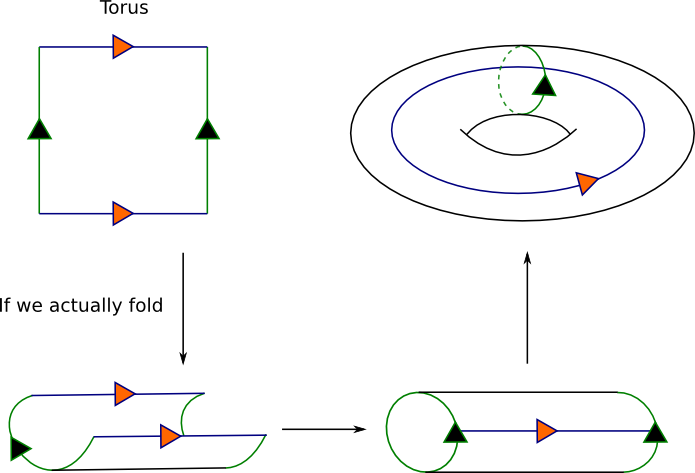
\includegraphics[width=\textwidth]{figures/part1.png}
            \captionof{figure}{Entstehung des Torus als Quotientenraum von $[0,1]^2$. \\
\tiny Quelle: \href{http://3.bp.blogspot.com/_swn7VcF-Vqc/TCpcMmi8qII/AAAAAAAAAHw/3QtMkZsikpY/s1600/part1(6).png}{http://3.bp.blogspot.com/\_swn7VcF-Vqc/TCpcMmi8qII/AAAAAAAAAHw/3QtMkZsikpY/s1600/part1(6).png}}
            \end{minipage} \\ \\
        \item Sei $X = [0,1] ^2 \subset \R^2$. Identifizieren wir $(t,0) \sim  (t,1)$ sowie $(0,s) \sim  (1, 1-s)$, so erhalten wir die \vocab{Kleinsche Flasche}. 
            \begin{minipage}{\textwidth}
                \begin{minipage}{0.3\textwidth}
                        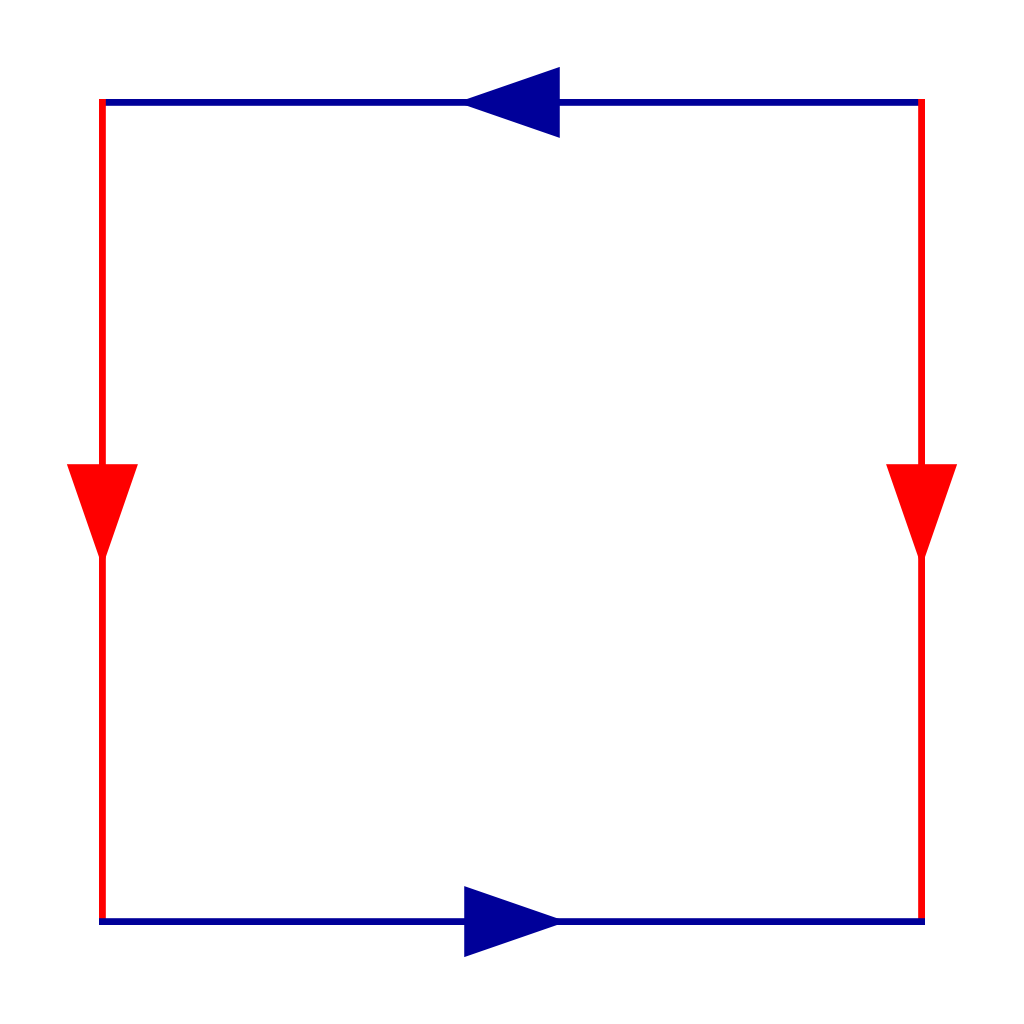
\includegraphics[width=\textwidth]{figures/1024px-Klein_Bottle_Folding_1.svg.png}
                \end{minipage}
                \begin{minipage}{0.3\textwidth}
                    \centering
                    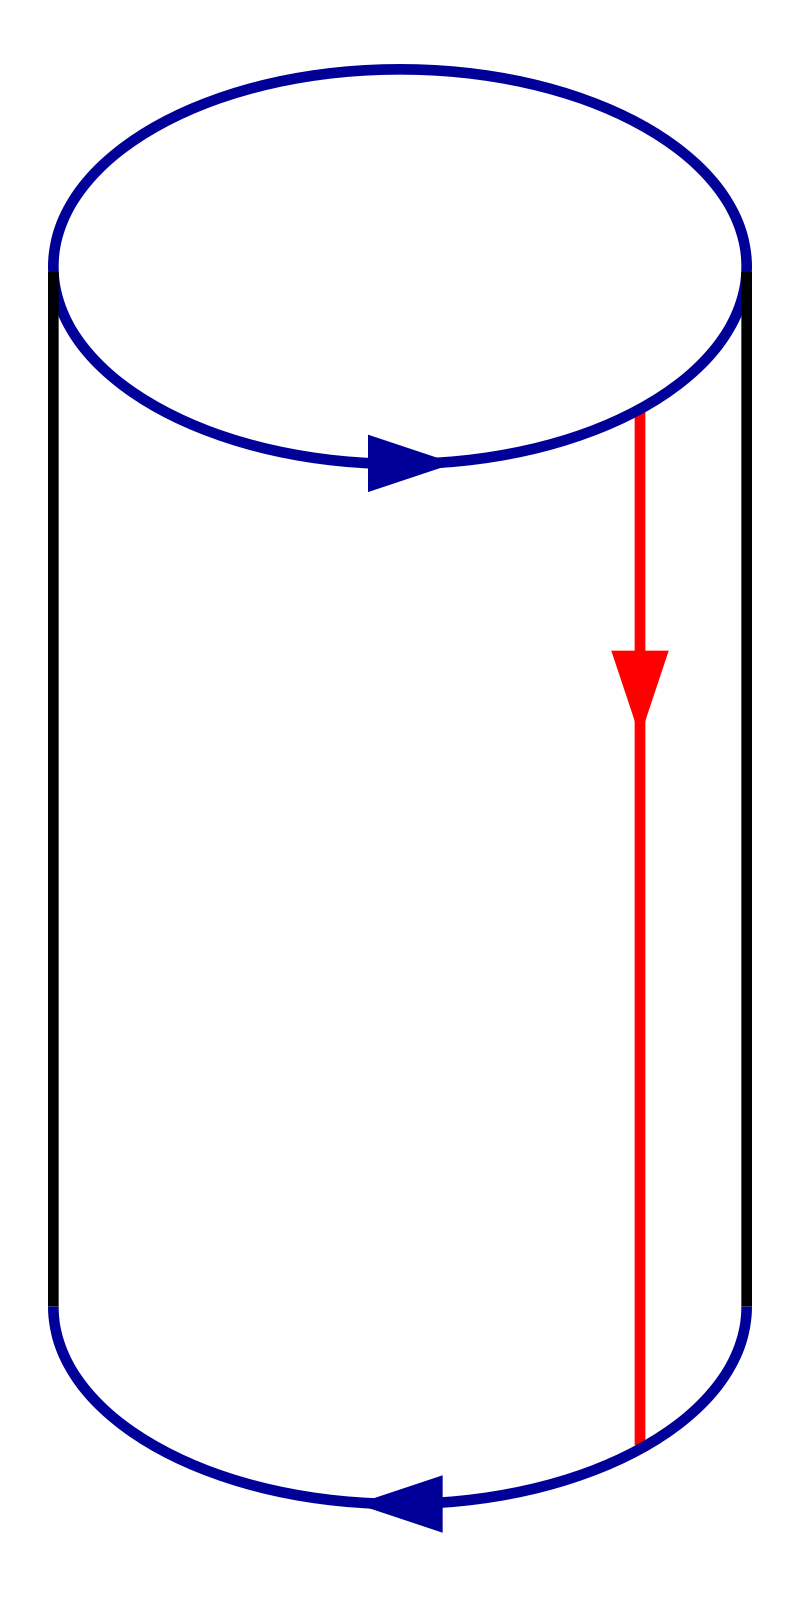
\includegraphics[width=0.6\textwidth]{figures/800px-Klein_Bottle_Folding_2.svg.png}
                \end{minipage}
                \begin{minipage}{0.3\textwidth}
                    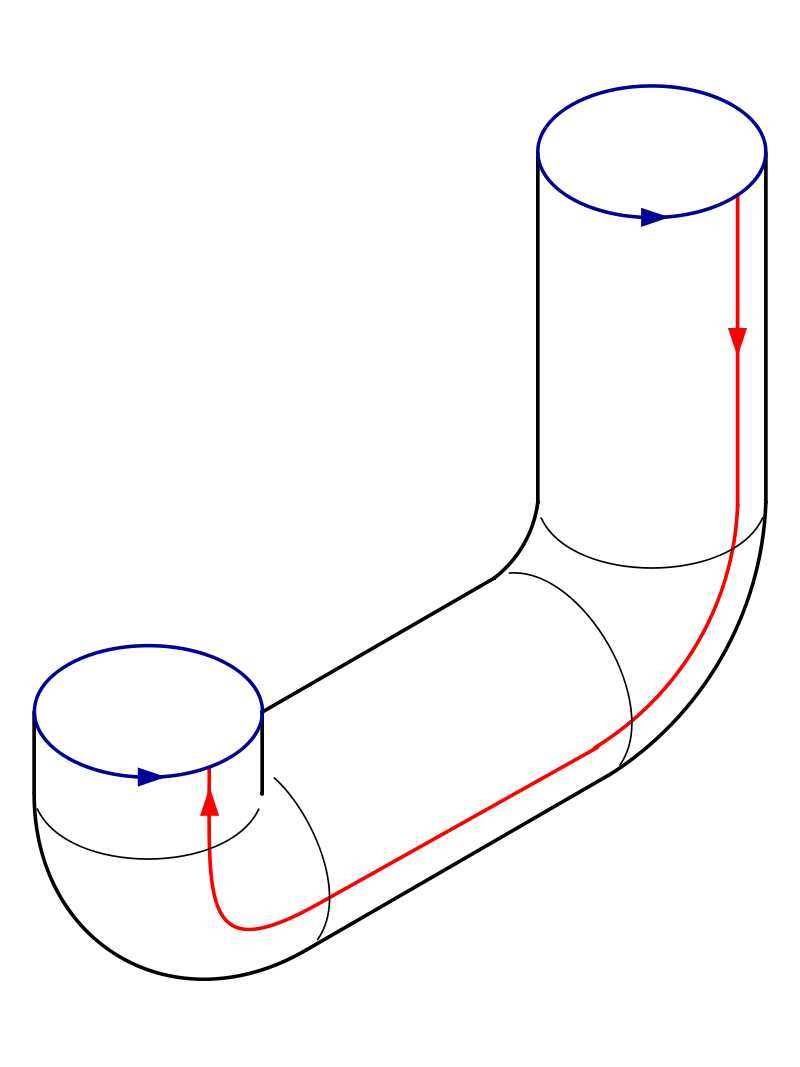
\includegraphics[width=\textwidth]{figures/800px-Klein_Bottle_Folding_3.svg.png}
                \end{minipage}
                \\
                \begin{minipage}{0.3\textwidth}
                    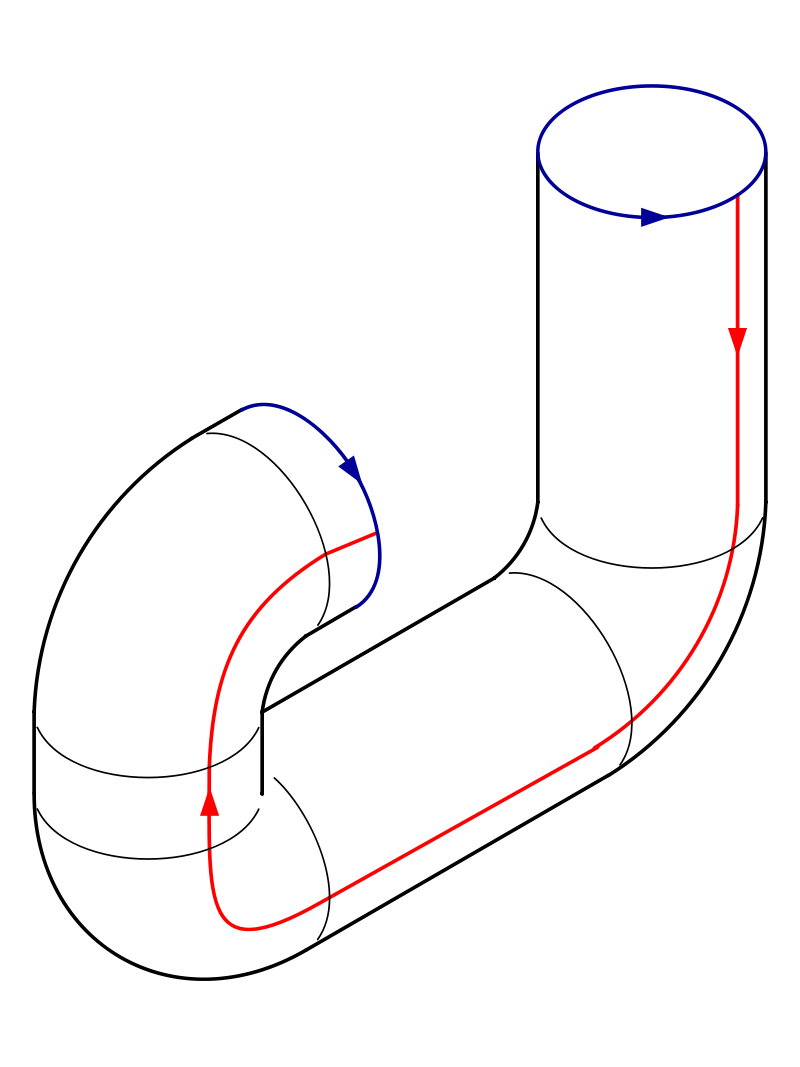
\includegraphics[width=\textwidth]{figures/800px-Klein_Bottle_Folding_4.svg.png}
                \end{minipage}
                \begin{minipage}{0.3\textwidth}
                    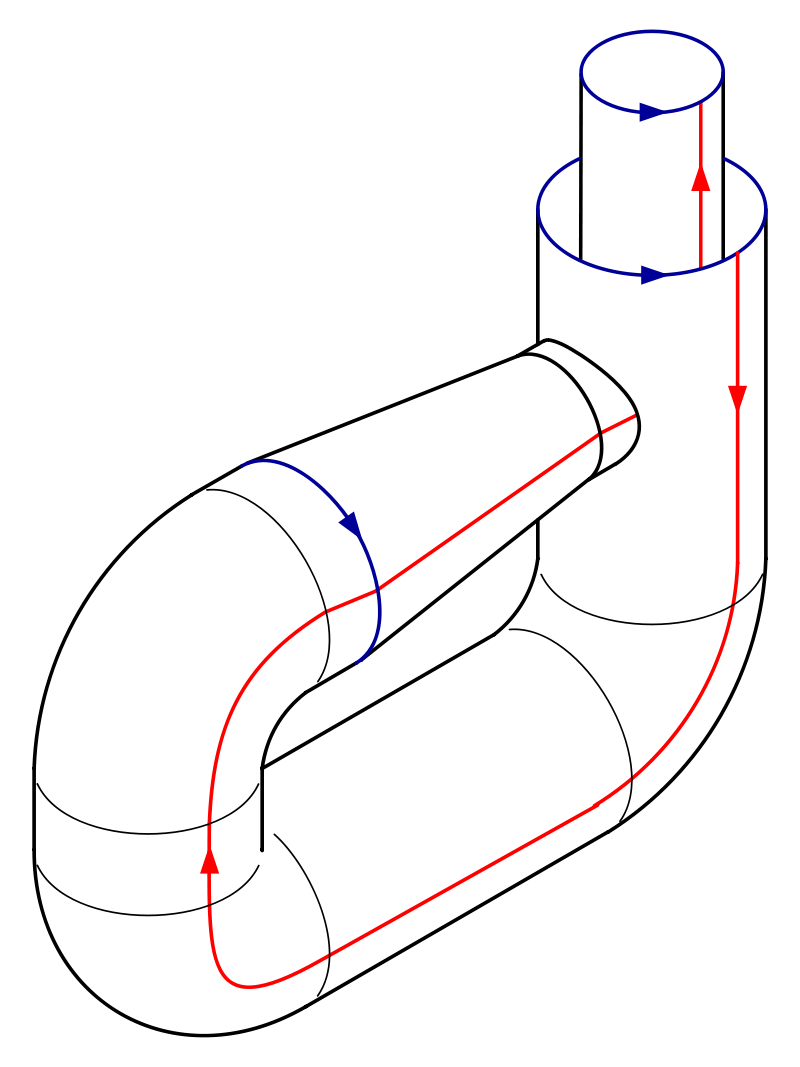
\includegraphics[width=\textwidth]{figures/800px-Klein_Bottle_Folding_5.svg.png}
                \end{minipage}
                \begin{minipage}{0.3\textwidth}
                    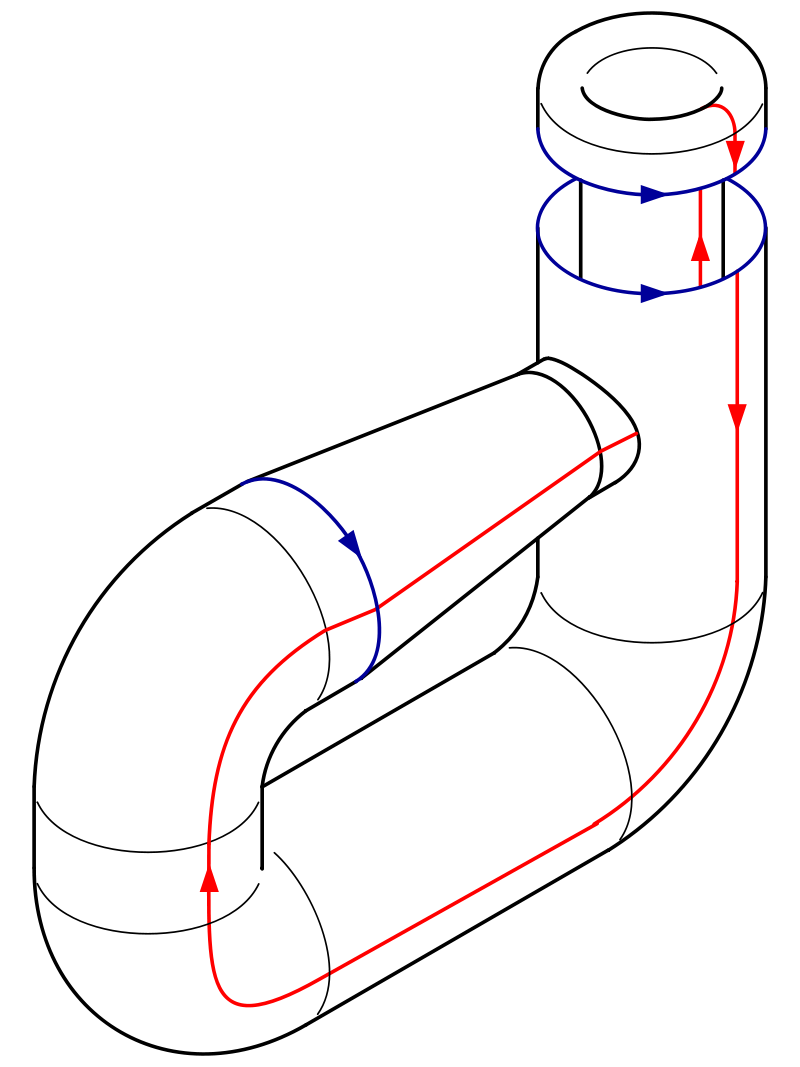
\includegraphics[width=\textwidth]{figures/800px-Klein_Bottle_Folding_6.svg.png}
                \end{minipage}
                \\
                \begin{minipage}{\textwidth}
                    \captionof{figure}{Entstehung der Kleinschen Flasche als Quotientenraum von $[0,1]^2$. \\ \tiny Quelle: \href{https://commons.wikimedia.org/wiki/File:Klein_Bottle_Folding_1.svg}{https://commons.wikimedia.org/wiki/File:Klein\_Bottle\_Folding\_1.svg}}
                \end{minipage}
            \end{minipage}
        \item Betrachte auf dem $\R^{n+1}\setminus \left \{0\right\} $ die Relation $x \sim  λx$ für $λ>0\in \R$. Dann ist $\R^{n+1} / \sim  \cong S^n$. Zunächst ist nämlich die Abbildung
                \begin{equation*}
                f: \left| \begin{array}{c c l} 
                \R^{n+1}\setminus \left \{0\right\}  & \longrightarrow & S^n \\
                x & \longmapsto &  \frac{x}{\lVert x \rVert _2}
                \end{array} \right.
            \end{equation*}
            stetig und die induzierte Abbildung $\R^{n+1} \setminus \left \{0\right\}  / \sim \to  S^n$ ist bijektiv. Das rechnen wir nach: Seien $x\neq y$ mit $d(x,y) < \delta$, so ist:
            \begin{equation}
                \begin{split}
                    d\left( \frac{x}{\lVert x \rVert },\frac{y}{\lVert y \rVert } \right) &\leq d\left( \frac{x}{\lVert x \rVert },\frac{y}{\lVert x \rVert } \right) + d\left( \frac{y}{\lVert x \rVert },\frac{y}{\lVert y \rVert } \right)  \\
                                                                                          &= \frac{1}{\lVert x \rVert } d(x,y) + \sqrt{\sum \left( \frac{y_i}{\lVert x \rVert }-\frac{y_i}{\lVert y \rVert } \right)^2 }  \\
                                                                                          &= \frac{1}{\lVert x \rVert } d(x,y) + \sqrt{\frac{(\lVert x \rVert -\lVert y \rVert )^2}{\lVert x \rVert \lVert y \rVert }} \lVert y \rVert \\
                                                                                          &< \frac{1}{\lVert x \rVert }\cdot \delta + \frac{\delta}{\lVert x \rVert ^2 + \delta \lVert x \rVert }(\lVert x \rVert +\delta) \to  0
                \end{split}
            \end{equation}
            also ist $f$ stetig. Mit der Inklusion  $ι: S^n \to  \R^{n+1} \setminus \left \{0\right\} $ erhalten wir
            \[
            f \circ  ι = \id_{S^n}
            .\] 
            Übung: Daraus folgt bereits, dass $S^n$ die Quotiententopologie trägt.
        \item Setzen wir erneut $X = \R^{n+1} \setminus \left \{0\right\} $, aber diesmal $x \sim  \lambda x$ für $λ\in \R \setminus  \left \{0\right\} $, so heißt der Quotient
            \[
            X / \sim  =: \R P^n
            .\] 
            der \vocab[Raum!reell projektiv]{reelle projektive Raum}.  Es ist
            \[
                \R P^n \cong S^n / (x \sim -x)
            .\] 
            Dies sehen wir mittels folgendem Diagramm:
            \begin{equation}
            \begin{tikzcd}
                \R^{n+1} \setminus \left \{0\right\}  \ar[two heads]{d} \ar[shift left]{r}{f} & S^n \ar[shift left]{l}{ι} \ar[two heads]{d} \\
                \R P^n \ar[dashed, shift left]{r}{\overline{f}} & S^n / (x \sim  - x) \ar[dashed, shift left]{l}{\overline{ι}}
            \end{tikzcd}
            \end{equation}
            Die Abbildungen $\overline{ι}$ und $\overline{f}$ sind stetig nach der universellen Eigenschaft und invers zueinander. \\
            \begin{minipage}{\textwidth}
                \centering
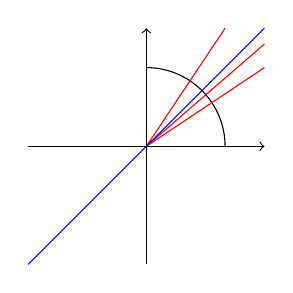
\begin{tikzpicture}
    \draw[->] (-1.5,0) -- (1.5,0);
    \draw [->] (0,-1.5) -- (0,1.5);
    \draw (1,0) arc (0:90:1);
    \draw[red] (0,0) -- (1.5,1);
    \draw[red] (0,0) -- (1.5,1.3);
    \draw[red] (0,0) -- (1,1.5);
    \draw[blue] (-1.5,-1.5) -- (1.5,1.5);
\end{tikzpicture}
\captionof{figure}{Konstruktion des reellen projektiven Raums für den Fall $n=1$. Wir identifizieren die roten Strahlen miteinander, nicht jedoch den gesamten blauen, da $λ>0$.}
            \end{minipage}
            \\ 
        \item Sei $X$ ein topologischer Raum und  $A\subset X$ eine Teilmenge. Definiere die Relation $\sim $ durch $a\sim a'$ für $a,a'\in A$ (bzw. erzeuge eine dadurch). Dann setzen wir
            \[
            X / A := X / \sim 
            .\] 
            Es ergibt sich
            \begin{itemize}
                \item $[0,1] / \left \{0,1\right\} \cong S^1$ 
                \item $[0,1] / [0,1)$ hat zwei Punkte  $[0,1)$ und  $\left \{1\right\} $. Es ist $[0,1) \subset [0,1]$ offen, aber $\left \{1\right\} $ nicht, also handelt es sich um den Sierpinski-Raum.
            \end{itemize}
    \end{enumerate}
\end{example}
\begin{remark}
    Quotientenräume von metrischen Räumen sind im Allgemeinen nicht metrisierbar.
\end{remark}




\section{Trennungsaxiome}
\begin{definition}[Hausdorff'sch]\label{def:hausdorff}
    Ein topologischer Raum heißt \vocab[Topologischer Raum!Hausdorff]{Hausdorff} (oder \vocab[Topologischer Raum!Hausdorff'sch]{Hausdorffsch}), wenn $\forall x,y\in X$ mit $x\neq y$ offene Mengen $U_x, U_y\subset X$ existieren mit $x\in U_x$ und $y\in U_y$, sodass $U_x \cap U_y = \emptyset$. Diese Eigenschaft heißt auch Trennungsaxiom\index{Trennungsaxiom} \vocab[Trennungsaxiom!$T_2$]{$T_2$}. \\
    \begin{minipage}{\textwidth}
    \centering    
\begin{minipage}{0.3\textwidth}
        \centering
        \incfig{hausdroff-raum}
    \end{minipage}
    \end{minipage}
\end{definition}

\begin{theorem}\label{thm:metrisierbarer-raum-ist-hausdorff}
    Ist $X$ metrisierbar, so ist  $X$ Hausdorffsch.
\end{theorem}
\begin{proof}
    Sei $d$ eine Metrik auf  $X$, die die Topologie induziert. Seien  $x,y\in X$ mit $x\neq y$. Setze
    \[
        U_x := U\left( x, \frac{d(x,y)}{2} \right) \qquad U_y = U\left( y, \frac{d(x,y)}{2} \right) 
    .\] 
    Dann ist $U_x \cap U_y = \emptyset$, denn für alle $z\in U_x \cap U_y$ ist
    \[
        d(x,y) \leq  d(x,z) + d(z,y) < \frac{d(x,y)}{2} + \frac{d(x,y)}{2} = d(x,y)
    .\] 
    , was nicht sein kann.
\end{proof}
\begin{example}
    $\R^n$ ist Hausdorffsch.
\end{example}
\begin{theorem}\label{thm:hausdorff-impliziert-t1}
    Ist $X$ Hausdorffsch und  $x\in X$, dann ist $\left \{x\right\} \subset X$ abgeschlossen.
\end{theorem}
\begin{proof}
    Für $y\neq x$ existiert $U_y$ offen mit  $x\not\in U_y$ und $y\in U_y$. Dann ist
    \[
    X \setminus \left \{x\right\}  = \bigcup_{y\neq x} U_y 
    .\] 
    offen. \\
\end{proof}
    \begin{minipage}{\textwidth}
        \centering
    \incfig{hausdorff-impliziert-t1}
    \captionof{figure}{Skizze zum Beweis von \autoref{thm:hausdorff-impliziert-t1}}
    \end{minipage}
\begin{remark}
    Ein topologischer Raum, für den alle $\left \{x\right\} $ abgeschlossen sind, heißt \vocab[Trennungsaxiom!$T_1$]{$T_1$-Raum}.
\end{remark}
\begin{remark*}
    Man findet in der Literatur auch folgende Definition: \\
    Ein topologischer Raum heißt $T_1$-Raum, wenn es für je zwei verschieden Punkte $x\neq y$ Umgebungen $U_x,U_y$ gibt mit  $x\in U_x, y\in U_y$ und $x\not\in U_y, y\not\in U_x$. \\
    Im Gegensatz zum Hausdorff-Raum trennen wir zwei Punkte also durch 2 nicht notwendigerweies offene Umgebungen. Mit dem gleichen Beweis wie in \autoref{thm:hausdorff-impliziert-t1} zeigen wir dann, dass jeder Punkt abgeschlossen ist. Ist umgekehrt $X$ ein Raum, in dem alle Punkte abgeschlossen sind, so können wir  $x,y$ stets durch die offenen Umgebungen  $y\in X \setminus \left \{x\right\} $ sowie $x\in X \setminus \left \{y\right\} $ trennen. Die beiden Definitionen sind also äquivalent.
    \begin{minipage}{\textwidth}
    \incfig{t1-raum}
    \captionof{figure}{Ein $T_1$-Raum}
    \end{minipage}
\end{remark*}



\begin{lemma}\label{lm:teilraum-von-hausdorffraum-ist-hausdorff}
    Sei $X$ Hausdorffsch und $A\subset X$ ein Teilraum. Dann ist auch $A$ Hausdorffsch.
\end{lemma}
\begin{proof}
    Sei $x\neq y\in A$. Dann existieren $U_x, U_y\subset X$ offen mit $x\in U_x$ und $y\in U_y$ sowie $U_x \cap U_y = \emptyset$. Dann sind
    \[
    U_x \cap A \qquad U_y \cap A \subset A
    .\] 
    offen in $A$ und erfüllen die Bedingungen.
\end{proof}


\begin{remark}
    Jeder diskrete Raum ist Hausdorffsch. Ist $X$ endlich und Hausdorffsch, so ist  $X$ diskret.
\end{remark}
\begin{proof}
    Für jedes $y\neq x$ existiert ein $U_x^y$ offen mit  $x\in U_x^y$ und $y\not\in U_x^y$. Dann ist aber
    \[
    \left \{x\right\}  = \bigcap_{y\neq x} U_x^{y}
    .\] 
    offen (da $X$ endlich), also ist $X$ diskret. Die Umkehrung ist offensichtlich.
\end{proof}
\begin{example}
    $S^n \subset \R^{n+1}$ ist Hausdorffsch.
\end{example}

\begin{definition}[Normal]\label{def:normal}
    Ein topologischer Raum heißt \vocab[Topologischer Raum!normal]{normal}, falls
    \begin{itemize}
        \item $X$ ist Hausdorffsch
        \item  $\forall A,B\subset X$ abgeschlossen mit $A \cap B = \emptyset$ existieren $U_A, U_B \subset X$ offen mit $A\subset U_A$, $B\subset U_B$ und $U_A \cap U_B = \emptyset$. Diese Eigenschaft heißt auch Trennungsaxiom \vocab[Trennungsaxiom!$T_4$]{$T_4$}. \\
            \begin{minipage}{\textwidth}
                \centering
                \begin{minipage}{0.3\textwidth}
    \incfig{normaler-raum}
                \end{minipage}
            \end{minipage}
    \end{itemize}
\end{definition}


\begin{remark}
    Manchmal gibt es diese Definition auch ohne Hausdorff'sch.
\end{remark}

\begin{theorem}\label{thm:metrischer-raum-ist-normal}
    Ist $X$ metrisierbar, dann ist  $X$ normal.
\end{theorem}

\begin{proof}
    Übung.
\end{proof}

\begin{definition}[Regulär]\label{def:regulär}
    Ein topologischer Raum $X$ heißt  \vocab[Topologischer Raum!regulär]{regulär}, falls $X$ Hausdorff ist und  $\forall  A \subset X$ abgeschlossen und $x\in X \setminus A$ existieren $U_a, U_{x}$ offen mit $A\subset U_A, x\in U_x$ und $U_A \cap U_x = \emptyset$. (Auch Trennungsaxiom \vocab[Trennungsaxiom!$T_3$]{$T_3$} genannt). \\
    \begin{minipage}{\textwidth}
        \centering
        \begin{minipage}{0.7\textwidth}
        \centering
        \incfig{regular-space}
        \end{minipage}
    \end{minipage}
\end{definition}

\begin{remark}
    Klarerweise gilt $T_4 \implies T_3$, d.h. jeder normale Raum ist auch regulär. Hierzu benötigen wir nur, dass Punkte in $T_4$-Räumen abgeschlossen sind, aber das folgt mit \autoref{thm:hausdorff-impliziert-t1}, bzw. damit, dass wir bereits $T_4 \implies T_2 \implies T_1$ wissen.
\end{remark}
\begin{figure}[ht]
    \centering
    \label{fig:regular-space}
\end{figure}


\section{Kompaktheit}
Aus der Analysis ist (vielleicht) folgender Satz bekannt.
\begin{theorem}[Heine-Borel]\label{thm:heine-borel}
    Für $X\subset \R^n$ sind äquivalent:
    \begin{enumerate}[1)]
        \item $X$ ist abgeschlossen und beschränkt.
        \item Jede offene Überdeckung von $X$ hat eine endliche Teilüberdeckung
    \end{enumerate}
\end{theorem}

\begin{recap}
    'Jede offene Überdeckung besitzt eine endliche Teilüberdeckung' bedeutet: \\
    Für jede Familie $\left \{U_i\right\} _{i \in I}$ mit $U_i \subset X$ offen und $X \subset \bigcup_{i \in I}U_i$ existiert eine endliche Teilmenge $J\subset I$ mit $X \subset \bigcup_{j\in J} U_j$
\end{recap}
\begin{proof}
    später.
\end{proof}

\begin{definition}[Kompaktheit]\label{def:kompakt}
    Ein topologischer Raum $X$ heißt  \vocab[Topologischer Raum!kompakt]{kompakt}, falls jede offene Überdeckung eine endliche Teilüberdeckung besitzt.
\end{definition}
\begin{remark}
    Manchmal heißt obige Definition auch quasi-kompakt, und kompakt bedeutet dann quasi-kompakt + Hausdorff.
\end{remark}

\begin{example}
   Die Räume
   \[
       [0,1] \subset \R \qquad S^n \subset \R^{n+1}
   .\] 
   sind beide kompakt (nach \ref{thm:heine-borel})
\end{example}

    \lecture{4}{Do 22 Apr 2021 10:15}{}
\begin{example}
    Zur Frage von letzter Woche (wenn wir einen Hausdorff-Raum haben und eine Äquivalenzrelation, deren Klassen abgeschlossen sind, ist dann der Quotient wieder  Hausdorff?): Wähle auf $[0,1]$ die Relation erzeugt von
     \[
    \frac{1}{n} \sim  1 - \frac{1}{n}
    .\] 
    für alle $n\in \N_>0$. Betrachte dann die Abbildung: 
    \[
        [0,1] \twoheadrightarrow [0,1] / \sim 
    .\] 
    Punkturbilder sind endlich, also abgeschlossen. Aber der Raum $[0,1] / \sim $ ist nicht hausdorffsch, denn wri können die Punkte $0,1$ nicht trennen.
\end{example}
\begin{theorem}
    Sei $X$ ein kompakter Raum und  $Y\subset X$ abgeschlossen. Dann ist $Y$ kompakt.
    \label{thm:closed-subset-of-compact-space-is-compact}
\end{theorem}
\begin{proof}
    Sei $\left \{U_i\right\} _{i \in I}$ eine offene Überdeckung von $Y$. Dann existieren $U_i' \subset X$ offen mit $U_i = U_i' \cap Y$. Die Familie
     \[
    \left \{U_i'\right\} _{i \in I}\cup \left \{\underbrace{X \setminus Y}_{\text{offen}}\right\} 
    .\] 
    ist nun eine offene Überdeckung von $X$. Dann existiert $J\subset I$ endlich, so dass
    \[
    \left \{U_j'\right\} _{j\in J} \cup \left \{X \setminus Y\right\} 
    .\] 
    die Menge $X$ überdeckt. Also ist  
    \[
        \left \{\underbrace{U_j' \cap Y}_{U_j}\right\} _{j\in J} \cup \left \{\underbrace{X \setminus Y \cap Y}_{=\emptyset}\right\}  
    \]
    eine endliche Überdeckung für $Y$.
\end{proof}
\begin{theorem}
    Sei $X$ ein Hausdorff-Raum und  $Y\subset X$ kompakt. Dann ist $Y$ abgeschlossen.
    \label{thm:compact-subset-of-hausdorff-space-is-closed}
\end{theorem}

\begin{corollary}
    Ist $X$ kompakt und Hausdorffsch, dann sind äquivalent:
    \label{thm:compact-iff-closed}
\begin{enumerate}[1)]
        \item $Y\subset X$ ist abgeschlossen
        \item $Y$ ist kompakt.
    \end{enumerate}
\end{corollary}
\begin{lemma}
    Sei $X$ ein Hausdorff Raum und  $Y\subset X$ kompakt. Dann existiert $\forall x\in X\setminus Y$ offene Teilmengen $U_{x,Y}$ und $V_{x,Y}$ von $X$ so dass:  $x\in U_{x,Y}$ und $Y\subset V_{x,Y}$ und $U_{x,Y} \cap V_{x,Y} = \emptyset$.
    \label{lm:compact-set-in-hausdorff-space-is-closed}
\end{lemma}
\begin{proof}
    Sei $x\in X\setminus Y$. $\forall y\in Y$ existieren $U_{x,y}$ und $V_{x,y}$ offen mit $x\in U_{x,y}$ und $y\in V_{x,y}$, weil $X$ Hausdorffsch. \\
    Dann ist  $\left \{V_{x,y} \cap Y\right\} _{y\in Y}$ eine offene Überdeckung von $Y$. Also existiert endliche Teilüberdeckung (da  $Y$ kompakt) induziert durch Punkte  $y_1,\ldots,y_n$. Also:
    \[
    Y\subset \bigcup_{i=1}^n V_{x,y_i}
    .\] 
    Sei
    \[
    V_{x,Y} := \bigcup_{i=1}^n V_{x,y_i} \qquad U_{x,Y} := \bigcap_{i=1}^n U_{x,y_i} 
    .\] 
    Es ist auch $x\in U_{x,Y}$, weil $x\in U_{x,y_i}$ für jedes $i$. Wir müssen also noch Disjunktheit prüfen, es ist:
     \[
    U_{x,Y} \cap V_{x,y_i} \subset U_{x,y_i} \cap V_{x,y_i} = \emptyset
    .\] 
    Also auch
    \[
        \emptyset=    U_{x,Y} \cap \bigcup_{i=1}^n V_{x,y_i} = U_{x,Y} \cap V_{x,Y}
    .\]
\end{proof}
    \begin{figure}[H]
    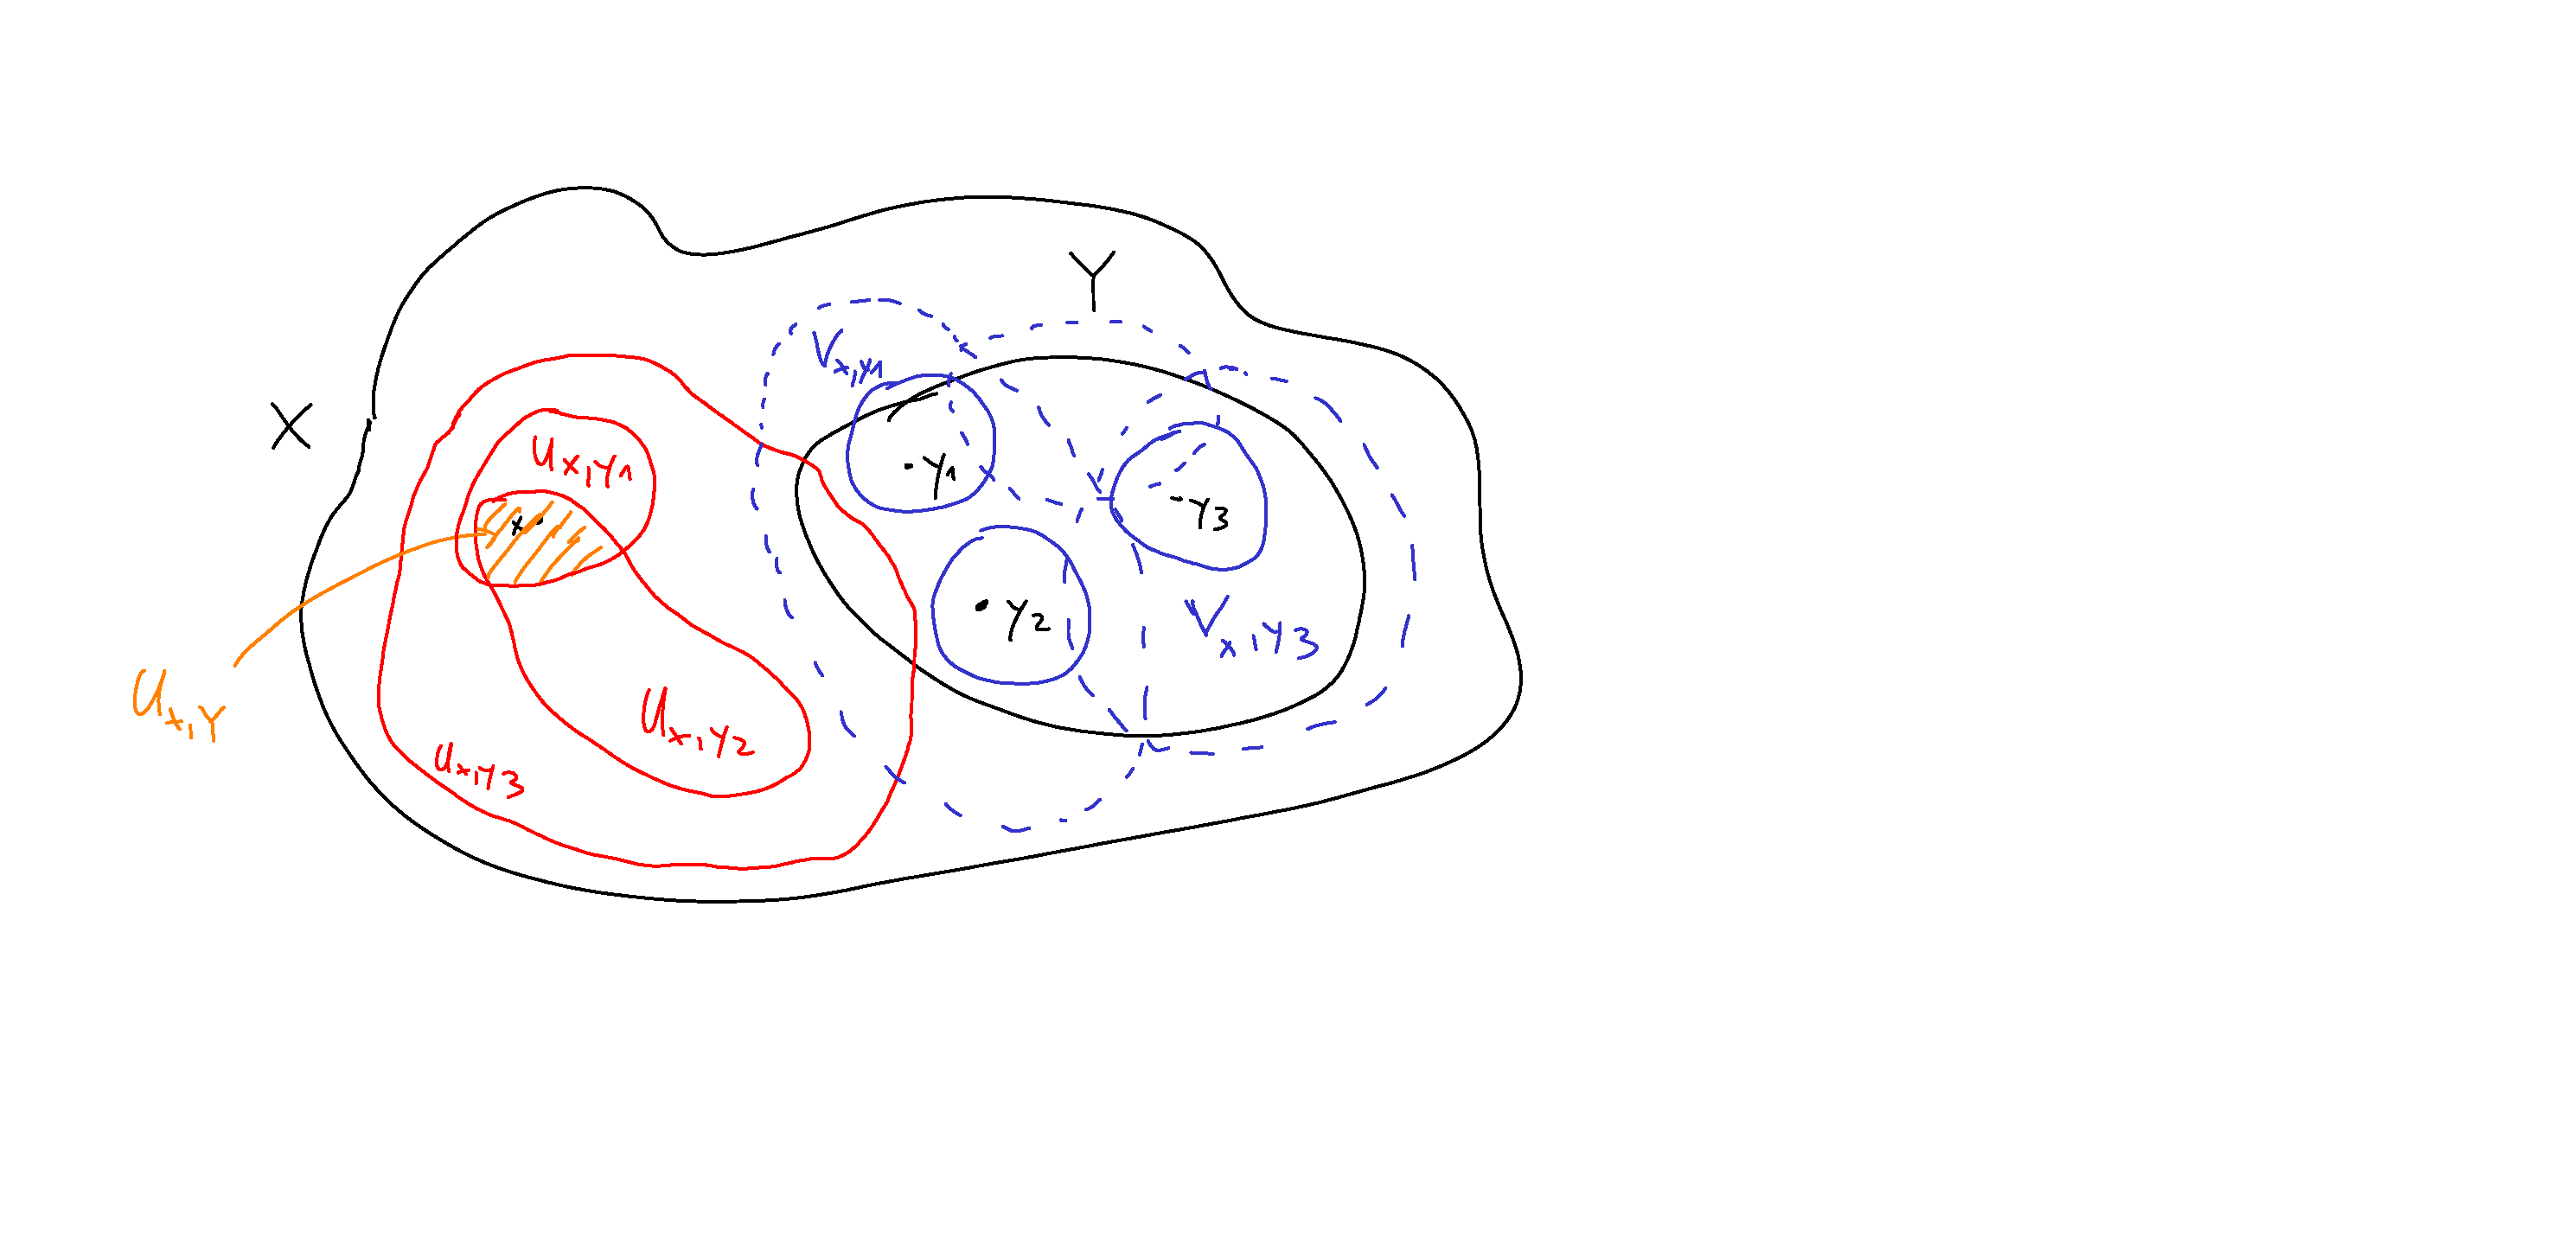
\includegraphics[scale=0.4]{figures/Lemma5.5.pdf}
    \caption{Skizze zum Beweis von Lemma \ref{lm:compact-set-in-hausdorff-space-is-closed}}
\end{figure}
\begin{proof}[Beweis von \ref{thm:compact-subset-of-hausdorff-space-is-closed}]
    Nach dem Lemma existieren $\forall x\in X \setminus Y$ ein $U_{x,Y}$ mit $x\in U_{x,Y}$ und $U_{x,Y} \cap Y = \emptyset$. Also ist
    \[
    X \setminus Y = \bigcup_{x\in X \setminus Y} U_{x,Y}
    .\] 
    offen und somit ist $Y$ abgeschlossen.
\end{proof}


\begin{example}['Gegenbeispiel' zu Satz \ref{thm:compact-subset-of-hausdorff-space-is-closed}]
    Sei $G$ die Gerade mit zwei Urpsrüngen: \\
    Betrachte  $\R\cup \left \{0'\right\} $ mit $U$ Umgebung von  $a\in \R$ falls $\exists ε>0$ mit $(a-ε, a+ε)\subset U$ und $U$ Umgebung von  $0'$ und  $U$ Umgebung von  $0'$, falls  $\exists ε>0$ mit $(-ε,0 \cup (0,ε) \subset U$ und $0' \in U$. \\
    Wir können uns gewissermaßen  $0,0'$ gleichberechtigt vorstellen, nur dass die beiden Punkte verschieden sind. \\
    Dann ist  $[-1,1] \subset G$ kompakt (Übung!), aber nicht abegschlossen, da $0' \in G \setminus [-1,1]$ ist, dies aber keine Umgebung von $0'$ ist.
    \begin{figure}[H]
        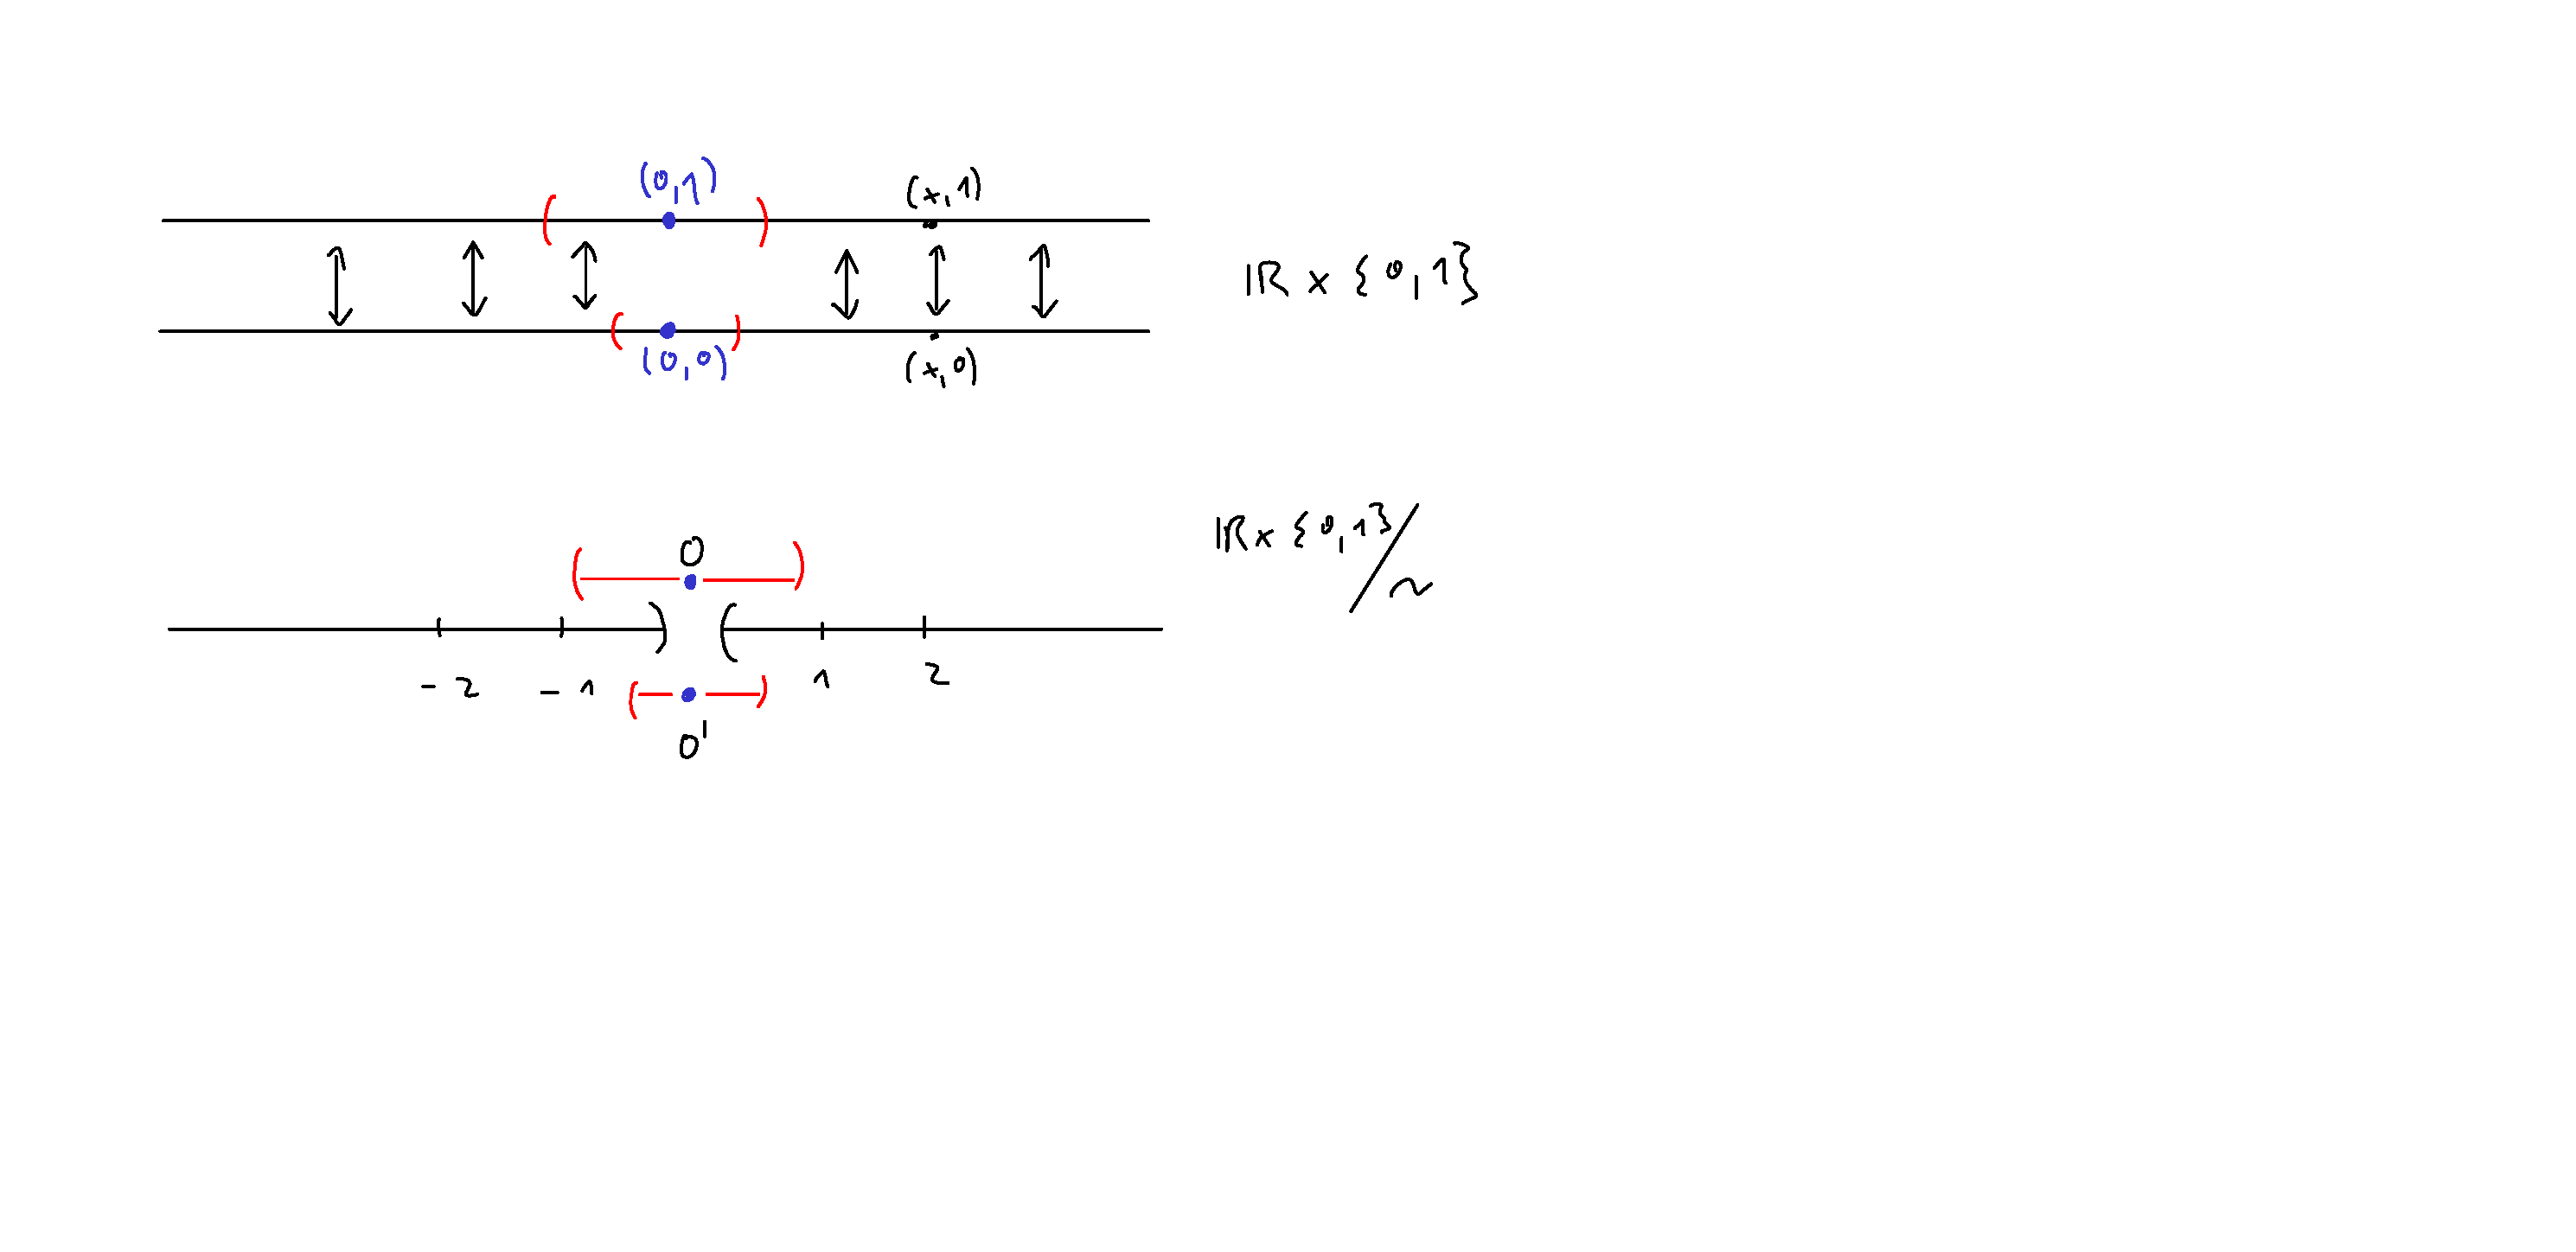
\includegraphics[scale=0.4]{figures/line-with-2-origins.pdf}
    \caption{Gerade mit 2 Ursprüngen}
    \end{figure}
\end{example}


\begin{proof}[Beweis von Satz \ref{thm:heine-borel}]
    '$2) \implies 1)$'. Sei $X\subset \R^n$ kompakt. Dann ist sie abgeschlossen nach \ref{thm:compact-subset-of-hausdorff-space-is-closed}. Zudem ist $X\subset \bigcup_{x\in X} U(x,1)$ eine offene Überdeckung. Da $X$ kompakt finden wir endlich viele  $x_1,\ldots,x_n\in X$ mit
    \[
        X \subset \bigcup_{i=1}^n U(x_i,1)
    .\] 
    Also ist
    \[
        \diam(X) \leq  \max \left \{d(x_i,x_j)\right\} +2 < \infty
    .\] 
    und somit ist $X$ auch beschränkt. \\
    ' $1)\implies 2)$'. Da $X$ beschränkt ist,  $\exists m>0$ mit $X\subset [-m,m]^n\subset \R^n$. Da $X$ abgeschlossen ist, genügt es nach \ref{thm:closed-subset-of-compact-space-is-compact} zu zeigen, dass  $[-m,m]^n$ kompakt ist. \\
    Wir führen einen Widerspruchsbeweis, nimm also an, dass  $[-m,m]^n$ nicht kompakt ist. Dann existiert eine offene Überdeckung  $\left \{U_i\right\} _{i \in I}$ ohne endliche Teilüberdeckung. \\
    Unterteile $[-m,m]^n$ in  $2^n$ gleich große Unterwürfel (halbiere jede Seite). Mindestens ein Unterwürfel hat keine endliche Teilüberdeckung. Unterteile diesen Würfel weiter und wähle wieder einen Unterwüfel, der keine endliche Teilüberdeckung hat. \\
    Wir erhalten eine Folge von Würfeln
     \[
         [-m,m]^n =     Q_0 \supset Q_1 \supset Q_2 \supset Q_3 \supset \ldots
    .\] 
    die jeweils keine endliche Teilüberdeckung durch $U_i's$ besitzen. \\
    Sei  $x_i \in Q_i$ beliebig. Dann ist $x_i$ eine Cauchy-Folge, also existiert $x = \lim_{i\to \infty} x_i$, und $x\in Q_0$, da $Q_0$ abgeschlossen. \\
    Somit gibt es ein $U_j$ mit  $x\in U_j$, da die $\left \{U_i\right\} _{i \in I}$ eine Überedeckung von $Q_0$ waren. Damit ist auch $U(x,ε) \subset U_j$ für ein $ε>0$. Wähle einen Würfel $x\in Q_k$ mit Kantenlänge $< \frac{ε}{\sqrt{n} }$, dann ist auch $Q_k \subset U(x,ε) \subset U_j$. Das ist aber ein Widerspruch dazu, dass $Q_k$ keine endliche Teilüberdeckung hat, \contra. \\
    Also ist  $Q_0$ kompakt.
\end{proof}

\begin{theorem}
    Sei $f: X \to  Y$ stetig und surjektiv und $X$ kompakt. Dann ist auch  $Y$ kompakt. 
    \label{thm:image-of-compact-space-is-compact}
\end{theorem}
\begin{proof}
    Sei $\left \{U_i\right\} _{i \in I}$ offene Überdeckung von $Y$. Dann ist
     \[
         \left \{f^{-1}(U_i)\right\} _{i \in I}
    .\] 
    offene Überdeckung von $X$. Da  $X$ kompakt ist, gibt es  $J\subset I$ endlich mit $X = \bigcup_{j\in J} f^{-1}(U_j)$. Dann ist 
    \[
        Y = f(X) = \bigcup_{j\in J} f(f^{-1}(U_j)) = \bigcup_{j\in J} U_j
    .\] 
    Also existiert eine endliche Teilüberdeckung von $Y$.
\end{proof}
\begin{corollary}
    Sei $f: X \to  Y$ stetig, $X$ kompakt und  $Y$ Hausdorff. Dann ist  $f$ abgeschlossen, d.h. $\forall A\subset X$ abgesclhossen ist $f(A) \subset Y$ abgeschlossen.
\end{corollary}
\begin{proof}
    Sei $A\subset X$ abgeschlossen. Dann ist $A$ kompakt. Also ist  $f(A)$ kompakt. Also ist  $f(A)$ abgeschlossen
\end{proof}
\begin{corollary}
    Ist $f: X \to  Y$ stetig und bijektiv, $X$ kompakt und  $Y$ Hausdorff, dann ist  $f$ ein Homöomorphismus.
\end{corollary}
\begin{proof}
    Wir müssen zeigen, dass die Umkehrabbildung stetig ist. Dafür reicht es zu zeigen, dass $\forall A\subset X$ abgeschlossen auch $f(A) = (f^{-1})^{-1}(A)$ abgeschlossen ist. Das gilt nach vorherigem Korollar.
\end{proof}
\begin{corollary}
    Sei $f: X \to  Y$ stetig und surjektiv, $X$ kompakt und  $Y$ Hausdorffsch. Dann trägt  $Y$ die Quotiententopologie, d.h.  $U\subset Y$ offen genau dann, wenn $f^{-1}(U) \subset X$ offen.
\end{corollary}
\begin{proof}
    '$\implies$' folgt wegen Stetigkeit. \\
    '$\impliedby$' Ist $f^{-1}(U) \subset X$ offen, dann ist $f^{-1}(Y \setminus U ) = U \setminus f^{-1}(U)$ abgeschlossen in $X$, also folgt aus dem Korollar dass
     \[
         Y \setminus U \stackrel{\text{surj.}}{=}   f\left( f^{-1}\left( Y \setminus U \right)  \right) 
    .\] 
    abgeschlossen ist, also ist $U\subset Y$ offen.
\end{proof}
\begin{proof}[Satz 3.3]
    Schon gezeigt:
        \begin{equation*}
        \begin{array}{c c l} 
            [0,1] & \longrightarrow & S_1 \\
        t & \longmapsto &  2^{2\pi it}
        \end{array}
    \end{equation*}
    ist stetig und surjektiv und faktorisiert über
    \[
        [0,1] /\left \{0,1\right\}  \to  S^1
    .\] 
    mit $f$ stetig und bijektiv. Wir wissen nun:  $S^1$ ist Hausdorffsch und  $[0,1]$ ist kompakt. Nach Satz 5.5 ist auch  $[0,1] /\left \{0,1\right\} $ kompakt, also ist $f$ ein Homöomorphismus nach Korollar 5.8.
\end{proof}


\begin{theorem}
    Jeder kompakte Hausdorff-Raum ist normal.
\end{theorem}
\begin{proof}
    Seien $A,B\subset X$ abgeschlossen und disjunkt. Da $X$ kompakt ist, sind  $A,B$ kompakt. Nach Lemma 5.5 existieren  $\forall a\in A$ offene Mengen $U_a, V_a$ mit $a\in U_a, B\subset V_a$ und $U_a \cap V_a = \emptyset$. Dann ist
    \[
    A \subset \bigcup_{a\in A} U_a
    .\] 
    Also existieren $a_1,\ldots,a_n\in A$ mit
    \[
    A\subset \bigcup_{i=1}^n U_{a_i}
    .\] 
    wegen $A$ kompakt. Setze nun
    \[
    U_A := \bigcup_{i=1}^n U_{a_i}\supset A \qquad U_B := \bigcap_{i=1}^n V_{a_i}\supset B
    .\] 
$\forall i$ ist 
\[
    U_{a_i} \cap U_B \subset U_{a_i} \cap V_{a_i} = \emptyset
.\] 
und daraus folgt, dass
\[
U_A \cap U_B = \emptyset
.\] 
\end{proof}

\begin{theorem}
    Sei $X$ kompakt und Hausdorffsch, $q: X \to  Z$ surjektiv, wobei  $Z$ die Quotiententopologie trage. Dann sind äquivalent: 
    \begin{enumerate}[1)]
        \item $Z$ ist Hausdorffsch
        \item  $q$ ist abgeschlossen
    \end{enumerate}
\end{theorem}
\begin{proof}
    Die Richtung '$1) \implies 2)$' ist genau Korollar 5.7  \\
    '$2)\implies_1)$': Jedes $z\in Z$ hat ein Urbild $x\in X$ unter $q$. Es ist  $\left \{x\right\} \subset X$ abgeschlossen, da $X$ hausdorffsch. Wegen  $q$ abgeschlossen folgt nun, dass auch
    \[
        \left \{z\right\}  = q(\left \{x\right\} )
    .\] 
    abgeschlossen ist. Eine Teilmenge $W\subset X$ heißt \vocab{saturiert}, falls $W = q^{-1}(q(W))$ (insbesondere sind alle Urbilder saturiert, und $\iff  \forall x\in X \setminus W : g(x) \in Z \setminus g(W)$). \\
\begin{remark}
    Sei $U\subset X$ offen und saturiert, dann ist $q(U)$ offen. Hierzu schreibe
    \[
        U = q^{-1}(q(U)) \implies q(U) \text{ offen}
    .\] 
\end{remark}
Seien $y\neq z\in Z$. Dann sind $\left \{y\right\} ,\left \{z\right\} $ abgeschlossen und disjunkt. Dann sind auch
\[
    A = q^{-1}(y) \qquad B = q^{-1}(z)
.\] 
abgeschlossen und disjunkt (in  $X$). Nach Annahme ist  $X$ kompakt und Hausdorff, also normal nach Satz 5.10. Also existieren  $U_1,U_2\subset X$ offen mit $A\subset U_1,B\subset U_2$ und $U_1 \cap U_2 = \emptyset$. Setze
\[
    V_1 := X \setminus q^{-1}(q(X\setminus U_1)) \qquad V_2 := X \setminus q^{-1}(q(X\setminus U_2))
.\] 
\begin{claim}
    Es sind $V_1,V_2$ offen, disjunkt und saturiert und $A\subset V_1$ sowie $B\subset V_2$.
\end{claim}
\begin{proof}
    TODO
\end{proof}
Es folgt, dass $q(V_1),q(V_2)$ offen in $Z$ sind. Weiter ist  $y\in q(A)\subset q(V_1)$ und $z\in q(B) \subset q(V_2)$. Da $V_1,V_2$ disjunkt und saturiert, sind auch $q(V_1),q(V_2)$ disjunkt und wir sind fertig.
\end{proof}

    \lecture[Weiteres zum reellen projektiven Raum und zu kompakten Hausdorffräumen. Basen, Subbasen. Erzeugte Topologie. Satz von Alexander.]{Di 27 Apr 2021 12:16}{Basen, Subbasen}
\begin{proof}[Beweis der Behauptung]
    Es ist klar, dass $V_1, V_2$ offen sind. Für Disjunktheit sehen wir mit
    \[
        X \setminus U_i \subset  q^{-1}(q(X\setminus U_i))
    .\] 
    dass $U_i \supset X \setminus q^{-1}(q(X\setminus U_i)) = V_i$ 
    Für Saturiertheit genügt es zu sehen, dass $q^{-1}(C)$ saturiert ist für alle $C\subset Z$, da
    \[
        q^{-1}(q(q^{-1}(C))) = q^{-1}(C)
    .\] 
    weil $q$ surjektiv ist. Wegen
     \[
         \begin{split}
             A\subset U_1 &\implies X \setminus A \supset X \setminus U_1 \\ &\implies q(X\setminus A) \supset q(X\setminus U_1)\\ &\implies \underbrace{q^{-1}(q(X\setminus A))}_{=X\setminus A} \supset q^{-1}q(X\setminus U_1)
         \end{split}
    .\]
    liefert nun Komplementbildung unser gewnschtes Ergebnis, dass
    \[
        A \subset  X \setminus q^{-1}(q(X\setminus U_1)) = V_1
    .\] 
\end{proof}


\begin{example}
    $\R \mathbb{P}^n$ ist Hausdorffsch. 
    \begin{proof}
        Es ist $\R \mathbb{P}^n \cong S^n / x \sim  - x$. Sei
        \[
        q : S^n \to  S^n / x\sim -x
        .\] 
    \end{proof}
    die Projektion. Da $S^n$ kompakt und Hausdorffsch ist, ist  $\R \mathbb{P}^n$ Hausdorffsch genau dann, wenn $q$ abgeschlossen ist. Ist  $A\subset S^n$, so ist $q^{-1}(Q(A)) = A \cup -A$. \\
Da $-: S^n \to  S^n$ ein Homöomorphismus ist, ist $-A$ abgeschlossen, wenn  $A$ abgeschlossen ist. Dann ist auch  $A \cup -A$ abgeschlossen.
\end{example}
\begin{corollary*}[Projektiver Raum]\label{cor:reeller-projektiver-raum-ist-quotientenraum-von-dn}
    Sei $\sim $ auf $D^n = \left \{x \in \R^n \mid  \lVert x \rVert \leq 1\right\} $ erzeugt durch $x \sim -x$ für alle $x\in S^{n-1}\subset D^n$. Dann ist
    \[
    D^n / \sim  \cong \R \mathbb{P}^n
    .\] 
    Insbesondere ist 
    \[
        \R\mathbb{P}^1 \cong D^1 / \left \{-1,1\right\} \cong [0,1] / \left \{0,1\right\}  \cong S^1
    \]
    \label{cor:}
\end{corollary*}
\begin{proof}
    Betrachte die stetige Abbildung
        \begin{equation*}
        f: \left| \begin{array}{c c l} 
        D^n & \longrightarrow & S^n \\
        x& \longmapsto &  (x,\sqrt{1-\lVert x \rVert ^2}) 
        \end{array} \right.
    \end{equation*}
    \begin{equation*}
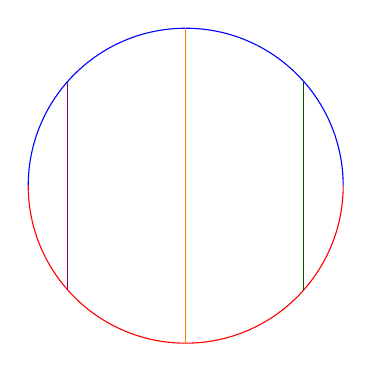
\begin{tikzpicture}
    \draw[red] (-2,0) arc (180:360:2);
    \draw[blue] (2,0) arc (0:180:2);
    \draw[green!30!black] (1.5,1.32) -- (1.5,-1.32);
    \draw[orange] (0,2) -- (0,-2);
    \draw[violet] (-1.5,1.32) -- (-1.5, -1.32);
\end{tikzpicture}
\qquad \qquad \qquad  
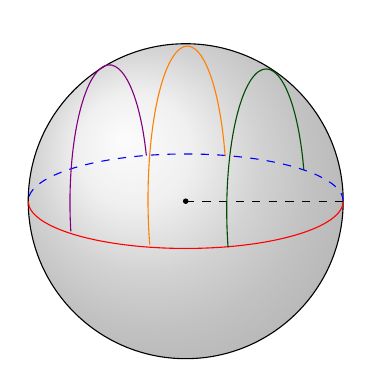
\begin{tikzpicture}
    \shade[ball color = gray!40, opacity = 0.4] (0,0) circle (2cm);
  \draw (0,0) circle (2cm);
  \draw[red] (-2,0) arc (180:360:2 and 0.6);
  \draw[dashed,blue] (2,0) arc (0:180:2 and 0.6);
  \draw[dashed] (0,0 ) -- (2,0);
  \fill[fill=black] (0,0) circle (1pt);
  \draw[green!30!black] (1.5,0.39686) arc (16.699:195:0.5 and 1.8);
  \draw[orange] (0.5,0.58) arc (16.699:197:0.5 and 1.95);
  \draw[violet] (-0.5,0.58) arc (20:192: 0.5 and 1.75);
\end{tikzpicture}
    \end{equation*}
    Wir erhalten das Diagramm:
    \begin{equation*}
    \begin{tikzcd}
        D^n \ar{r} \ar{d} & S^n \ar{d} \\
    D^n / \sim \ar[dashed,swap]{r}{\overline{f}} & S^n / (x\sim -x) \cong \R\mathbb{P}^n
    \end{tikzcd}
    \end{equation*}
    Wir sehen leicht, dass $\overline{f}$ bijektiv ist. Da $D^n$ kompakt, ist auch  $D^n / \sim $ kompakt, und $\R\mathbb{P}^n$ ist Hausdorffsch, also handelt es sich um einen Homöomorphismus (mit \autoref{cor:stetige-bijektion-von-kompaktem-raum-in-hausdorff-raum-ist-homöomorphismus})
\end{proof}

\begin{corollary}\label{cor:quotientenraum-von-kompaktem-hausdorffraum-mit-teilmenge-ist-hausdorff-gdw-teilmenge-abgeschlossen}
    Sei $X$ kompakt und Hausdorffsch und  $A\subset X$. Dann sind äquivalent
    \begin{enumerate}[1)]
        \item $X / A$ ist Hausdorffsch
        \item  $A$ ist abgeschlossen.
    \end{enumerate}
\end{corollary}
\begin{proof}
    '$1)\implies_2)$'. Ist $X / A$ Hausdorffsch, so ist die einpunktige Menge $\left \{[A]\right\}$ abgeschlossen (nach \autoref{thm:hausdorff-impliziert-t1}). Also ist $q^{-1}(A) = A$ abgeschlossen nach Definition der Quotiententopologie. \\
    '$2)\implies 1)$' Nach \autoref{thm:quotientenraum-von-hausdorffraum-ist-hausdorff-gdw-projektion-abgeschlossen} genügt es zu zeigen, dass $q: X \to  X / A$ abgeschlossen ist. Für $B\subset X$ abgeschlossen ist, müssen wir also zeigen, dass $q(B)$ abgeschlossen ist, nach Definiton also, dass  $q^{-1}(q(B))\subset X$ abgeschlossen ist. Nun ist
    \[
        q^{-1}(q(B)) = \begin{cases}
            B & \text{falls } B\cap A = \emptyset \\
            B \cup A & \text{falls }B \cap  A \neq  \emptyset
        \end{cases}
    .\] 
    abgeschlossen, weil $A$ abgeschlossen ist. 
\end{proof}


\begin{example}
    \begin{enumerate}[a)]
        \item
Es ist $D^n / S^{n-1}$   Hausdorffsch. Alternativ können wir auch sehen, dass $D^n / S^{n-1} \cong S^n$ ist. Hierzu betrachte die Projektion:
    \begin{equation*}
    \begin{array}{c c l} 
    D^n & \longrightarrow & S^n \\
    x & \longmapsto &  \begin{cases}
        (2x, \sqrt{1-\lVert 2x \rVert ^2} & 0 \leq  \lVert x \rVert \leq \frac{1}{2}  \\
        \left( \frac{2-2\lVert x \rVert }{\lVert x \rVert }\cdot x, - \sqrt{1-(2-2\lVert x \rVert )^2}  \right) & \frac{1}{2} \leq  \lVert x \rVert  \leq 1
    \end{cases}
    \end{array}
\end{equation*}
Diese ist stetig, denn falls $\lVert x \rVert =\frac{1}{2}$ ist
\[
\frac{2-2\lVert x \rVert }{\lVert x \rVert } = \frac{2-1}{\frac{1}{2}} = 2
.\] 
und
\[
    \sqrt{1-\lVert 2x \rVert ^2} = \sqrt{1-1} =0 = - \sqrt{0} = -\sqrt{1-(2-2\lVert x \rVert )^2}  
.\] 
Ist $\lVert x \rVert =1$, so ist
 \[
\frac{2-2\lVert x \rVert }{\lVert x \rVert } = 0
.\] 
und somit ist $f(x) = (0,-1) \in \R^n \times \R$. Also faktorisiert $f$ über  $\overline{f} : D^n / S^{n-1} \to  S^n$. Wir sehen wieder leicht, dass $\overline{f}$ stetige Bijektion ist. Da $D^n / S^{n-1}$ kompakt und $S^n$ Hausdorffsch, folgt wieder, dass  $\overline{f}$ ein Homöomorphismus ist. \\
\item Wir erhalten nun eine Abbildung:
    \[
    \begin{tikzcd}
        S^n \ar{r}{q} & S^n / (x\sim -x) \cong \R\mathbb{P}^n \cong D^n / (x\sim -x) \ar{r} &  D^n / S^{n-1} \cong S^n
    \end{tikzcd}
\]
und diese ist im Allgemeinen \underline{kein} Homöomorphismus, denn jeder Punkt hat 2 Urbilder.
    \end{enumerate}
\end{example}
\todo{Abbildung skizzieren}

\def\Base{\mathcal{S}} %temporary
\section{Basen und Subbasen}
\begin{definition}[Basis]\label{def:basis}
    Sei $(X, \mathcal{O})$ ein topologischer Raum. Sei $\Base \subset \mathcal{O}$ eine Menge offener Mengen. Dann heißt $\Base$
    \begin{description}
        \item[\vocab{Basis}], falls $\forall U\subset \mathcal{O}$ existiert $S_i \in \Base$ mit $U = \bigcup_{i\in I} S_i$ 
        \item[\vocab{Subbasis}], falls $\forall U\in \mathcal{O}$ existieren $I, K_i$ endlich sowie  $S_k \in  \Base$ mit 
            \[
            U = \bigcup_{i\in I} \bigcap_{k\in K_i} S_k 
            .\] 
    \end{description}
\end{definition}
\begin{remark}
Ist     $\Base$ eine Basis, so ist $\Base$ eine Subbasis.
\end{remark}
\begin{example}
    Ist $(X,d)$ ein metrischer Raum, so ist
     \[
         \Base = \left \{U(x,ε) \mid  x\in X, ε>0\right\} 
    .\] 
    eine Basis der Topologie.
\end{example}
\begin{theorem}[Erzeugte Topologie]\label{thm:erzeugte-topologie}
    Sei $X$ eine Menge,  $\Base \subset \mathcal{P}(X)$ eine Menge von Teilmengen. Dann existiert genau eine Topologie auf  $X$, für die  $\Base$ eine Subbasis ist, nämlich:
     \[
    \mathcal{O} = \left \{U\subset X \mid  U = \bigcup_{i \in  I} \bigcap_{k\in K_i} S_k \text{ mit } \abs{K_i}<\infty, S_k \in  \Base  \right\} 
    .\] 
\end{theorem}
\begin{proof}
    Übung als \autoref{aufgabe-3.2}.
\end{proof}
\begin{dnotation}
    Wir nennen $\mathcal{O}$ die \vocab[Topologie!von $\Base$ erzeugte]{von $\Base$ erzeugte Topologie}.
\end{dnotation}

\begin{lemma}[Stetigkeit auf Subbasiselementen]\label{lm:stetigkeit-auf-subbasis}
    Sei $f: X \to  Y$ eine Abbildung zwischen topologischen Räumen, $\Base$ eine Subbasis von $Y$. Dann sind äquivalent:
    \begin{enumerate}[1)]
        \item $f$ ist stetig
        \item  $f^{-1}(S)$ ist offen für alle $S\in \Base$
    \end{enumerate}
\end{lemma}

\begin{proof}
    '$1) \implies 2)$' ist klar, da Subbasiselemente offen sind. \\
    '$2) \implies 1)$'. Sei $U \subset Y$ offen, dann $\exists K_i$ endlich und $S_k \in \Base$ mit
    \[
    U = \bigcup_{i \in  I} \bigcap_{k\in K_i} S_k
    .\] 
    Dann ist aber genau
    \[
        f^{-1}(U) = \bigcup_{i \in  I} \bigcap_{k\in K_i} \underbrace{f^{-1}(S_k)}_{\text{offen}} 
    .\] 
    offen, weil endliche Schnitte und beliebige Vereinigung offener Mengen offen sind. Also ist $f$ stetig.
\end{proof}

\begin{theorem}\label{thm:subbasis-ist-basis-wenn-schnitt-generiert-wird}
    Eine Subbasis $\Base$ von  $(X, \mathcal{O})$ ist eine Basis genau dann, wenn
    \[
    \forall S_1, S_2 \in \Base \;\exists S_i \in \Base \colon S_1 \cap S_2 = \bigcup_{i \in I} S_i
    .\] 
\end{theorem}


\begin{proof}
'$\implies$'    Da $S_1,S_2 \in \Base$ sind diese offen. Dann ist auch $S_1\cap S_2$ offen. Ist $\Base$ Basis, dann gibt es also  $S_i \in  \Base$ mit 
\[
S_1 \cap  S_2 = \bigcup_{i \in  I} S_i
.\] 
'$\impliedby$' Angenommen, $U\subset X$ ist offen und von der Form
\[
    U = \bigcup_{i \in  I} \left( \bigcap_{k\in K_i} S_k \right) 
.\] 
mit $K_i$ endlich und  $S_k \in  \Base$. Nach Annahme ist
\[
\bigcap_{k\in K_i} = \bigcup_{j\in J_i} S_j  
.\] 
und damit ist
\[
U = \bigcup_{i\in I} \bigcup_{j\in J_i} S_j  
.\] 
\end{proof}
\begin{remark*}
    Nach Annahme ist eigentlich erstmal der Schnitt von 2 Mengen die Vereinigung von $S_i$. Allerdings kann man dies per Induktion leicht auf  $n$ Teilmengen verallgemeinern, wenn wir
     \[
         \bigcap_{k=1}^n S_k = S_1 \cap  \bigcap_{k=2}^{n} S_k = S_1 \cap \bigcup_{i\in I} S_i = \bigcap_{i\in I} (S_i \cap S_k) = \bigcup_{i\in I} \bigcup_{j\in J_i} S_j  
    .\]
    für geeignete $S_i, S_j\in \Base$ schreiben.
\end{remark*}
\begin{theorem}[Satz von Alexander]\label{thm:alexander}
    Sei $X$ ein topologischer Raum und  $\Base$ eine Subbasis. Dann ist  $X$ kompakt genau dann, wenn jede Überdeckung durch Elemente aus  $\Base$ eine endliche Teilüberdeckung besitzt.
\end{theorem}
\begin{proof}
    '$\implies$' ist klar. \\
    '$\impliedby$' Angenommen, $X$ ist nicht kompakt, dann betrachte die Menge
     \[
    \mathcal{C} := \left \{U \mid  U \text{ offene Überdeckung \underline{ohne} endliche Teilüberdeckung}\right\} \neq \emptyset
    .\] 
    Es ist $\mathcal{C}$ partiell geordnet, indem wir $U\leq U'$ für $U\subset U'$ setzen. \\
    Ist $U_1\subset U_2\subset \ldots$ eine Kette, so ist $\bigcup_{U_i}\in \mathcal{C}$, denn
    \begin{itemize}
        \item Offenbar ist $\bigcup_{i \in  I} U_i$ eine offene Überdeckung.
        \item Hat $\bigcup_{i \in  I} U_i$ eine endliche Teilüberdeckung, so ist diese schon in einem $U_i$ enthalten, und damit enthielte auch dieses  $U_i$ bereits eine endliche Teilüberedckung \contra
    \end{itemize}
Wir können also das Lemma von Zorn anwenden, und somit existiert ein maximales Elment $U\in \mathcal{C}$.
\begin{claim}
    Ist $V\subset X$ offen und  $V\not\in U$, so hat $U\cup \left \{V\right\} $ eine endliche Teilüberdeckung
\end{claim}
\begin{subproof}
    Sonst wäre $U \cup \left \{V\right\} \in \mathcal{C}$ und somit wäre $U$ nicht maximal
\end{subproof}
\begin{claim}
    $U \cap \Base$ ist keine Überdeckung
\end{claim}
\begin{subproof}
    Sonst hätte $U$ eine endliche Teilüberedckung nach Annahme.
\end{subproof}
Wegen Behauptung 2 existiert $x\in X$, der nicht von $U \cap \Base$ überdeckt wird. Sei $W\in U$ mit $x\in W$. Da $W$ offen ist, folgt
 \[
W = \bigcup_{i \in  I} \bigcap_{k\in K_i} S_k
.\] 
mit $K_i$ endlich und  $S_k \in \Base$. Dann existieren also $S_1,\ldots,S_n$ mit 
\[
x \in  \bigcap_{i=1}^n S_i \subset W 
.\] 
Da $x$ nicht von  $U \cap \Base$ überdeckt wird, ist $S_i \not\in U$. Aus der ersten Behauptung wissen wir nun aber, dass es $U_1^i, \ldots, u_{n_i}^i \in U$ mit
\[
\left \{U_j ^i\right\} _{j=1}^n \cup \left \{S_i\right\}  \quad \text{ ist Überdeckung von } X
.\] 
Sei nun 
\[
\hat{U} := \left \{U_j ^i \mid  1\leq i\leq n, 1\leq j\leq n_i\right\} \subset U
.\] 
Für alle $i$ gilt also
 \[
X \subset \bigcup_{V\in \hat{U}} V \cup S_i 
.\] 
Also folgt
\[
X \setminus \bigcup_{V\in \hat{U}} V \subset S_i 
.\] 
und damit ist auch
\[
X\setminus \bigcup_{V\in \hat{U}} V \subset S_1 \cap \ldots \cap S_n \subset W \in U 
.\] 
Also ist $\hat{U}\cup \left \{W\right\} $ eine endliche Teilüberdeckung von $U$, \contra.
\end{proof}

    % end lectures
\end{document}
